\makeatletter
\def\input@path{{../}}
\makeatother

\documentclass[/main.tex]{subfiles}

\begin{document}
\graphicspath{{./pics/}{ch2/pics/}}

\onlyinsubfile{\textpages}
\chapter{Overview of the \MJD}

The \textsc{Majorana} Collaboration is studying \bb -decay in \Ge{76} and is currently operating an array of High Purity Germanium (HPGe) detectors called the \MJD\cite{mjd2014}.
The goal of the next generation of \znbb\ searches is a sensitivity to \mbb\ of $\sim15$~meV, which corresponds to a half-life sensitivity in \Ge{76} of $\sim10^{28}$~y.
To reach this goal, an exposure on the order of several tonne-years will be required, with background levels in the region of interest of the decay of $<0.1$~cts/FWHM-t-y, as shown in Figure~\ref{fig:sensitivity}.
\begin{figure}[h]
  \centering
  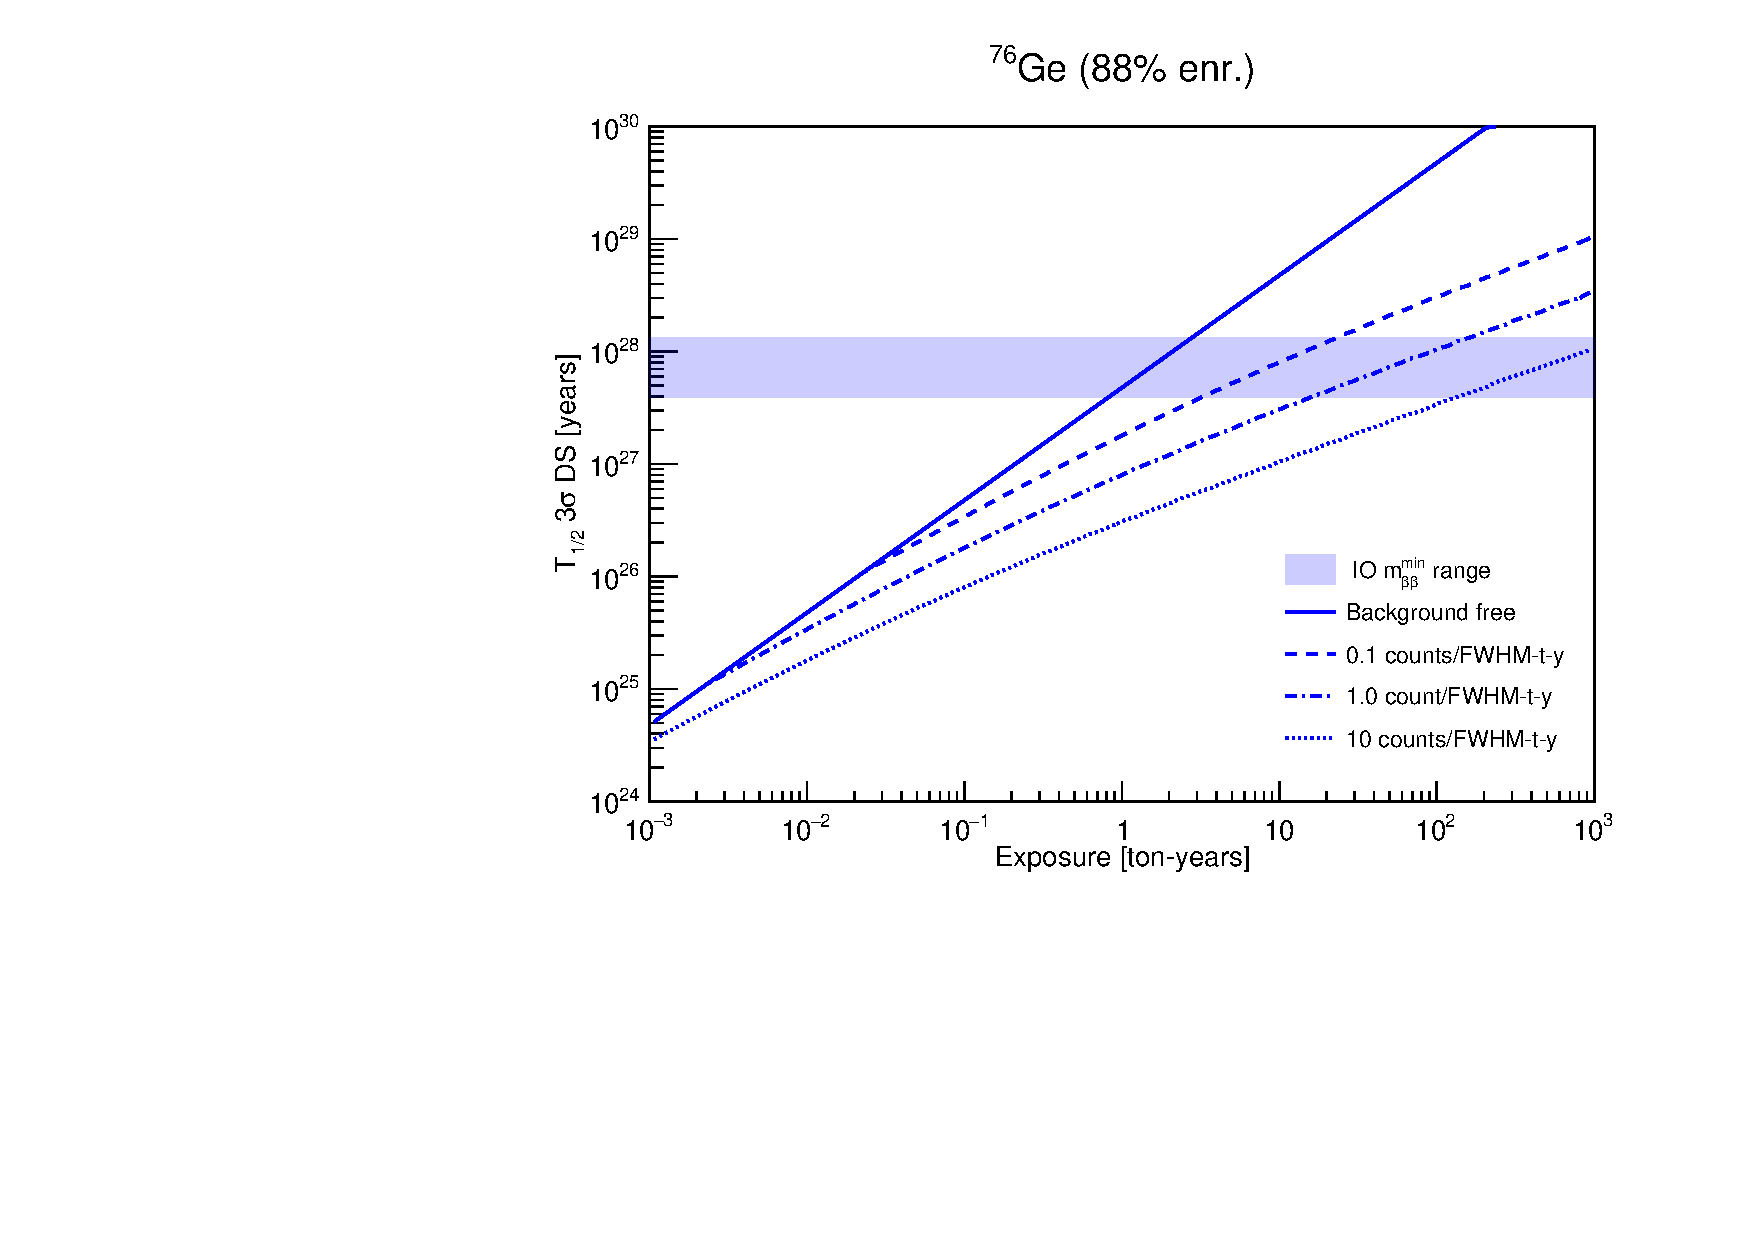
\includegraphics[width=0.8\textwidth]{sensitivityplot}
  \caption[Detection sensitivity to \znbb\ in \Ge{76}]{\label{fig:sensitivity}
    Detection sensitivity of a \znbb\ search in \Ge{76} as a function of isotopic exposure and the level of backgrounds in the region of interest. A blue band is drawn showing the next generation sensitivity goal. Image courtesy of Jason Detwiler.
  }
\end{figure}
With these future needs in mind, the \MJD\ was built with the following primary goals:
\begin{itemize}
\item Demonstrate backgrounds low enough to justify building \bb -decay experiment involving $\sim1$~tonne of \Ge{76}. The goal for the \MJD\ is a background rate of $<3$~background counts per tonne-year of isotopic exposure in a 4~keV region of interest around the 2039~keV Q-value of \znbb\ in \Ge{76}.
\item Demonstrate the scalability of the design and techniques of the \MJD\ towards a tonne-scale experiment.
\item Set competitive limits on the half-life of \znbb\ and on \mbb\ with other leading searches such as KamLAND-Zen and \Gerda \cite{kamlandzen, gerda}.
\item Search for additional physics beyond the Standard Model. This includes searches for bosonic dark matter, solar axions, Pauli exclusion principle violation, electron decay, lightly ionizing particles, and trinucleon decay\cite{mjdlowE2017, mjdlips2019, mjdtrinuc2019}. As discussed in Section~\ref{sec:bbestheory}, the search for \bbes\ has implications for some models beyond the standard model physics.
\end{itemize}
This chapter will describe the design of the \MJD\ and progress towards meeting these goals, with a focus on the most relevant elements of the experiment to the search for \bbes.

\section{Experimental Design}
The \MJD\ is using P-type Point Contact (PPC)\cite{Luke1989, Barbeau2007} HPGe detectors to search for \znbb.
PPC HPGe detectors are cylindrical semiconductor detectors that collect the positively charged electron holes at a small point-like contact with a diameter of a few mm.
This differs from the more common coaxial detector geometry, where both the electrons and holes are collected along much larger electrodes that extend coaxially along the detector.
The PPC geometry offers several advantages in performing a low background search for \znbb.
First, PPC HPGe detectors have intrisically low electronic noise due to a much lower capacitance than coaxial detectors.
This results in an improved energy resolution and lower energy thresholds.
Additionally, the PPC geometry enables pulse shape analysis (PSA) techniques to discriminate between single- and multi-site events.

\begin{figure}[h]
  \centering
  \subfloat[Natural Detector]{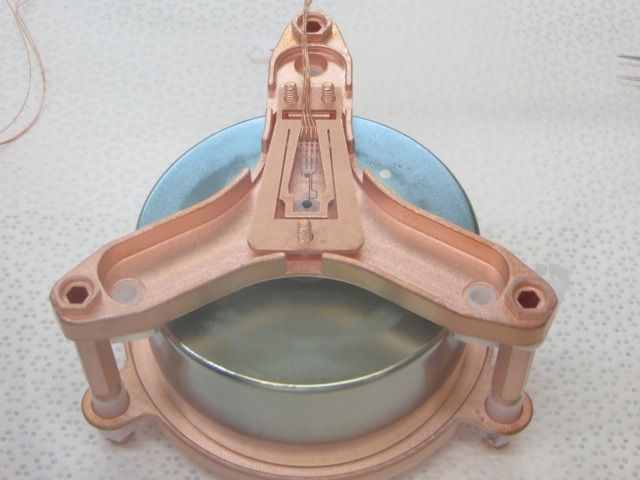
\includegraphics[height=6cm]{begedetector}}~
  \subfloat[Enriched Detector]{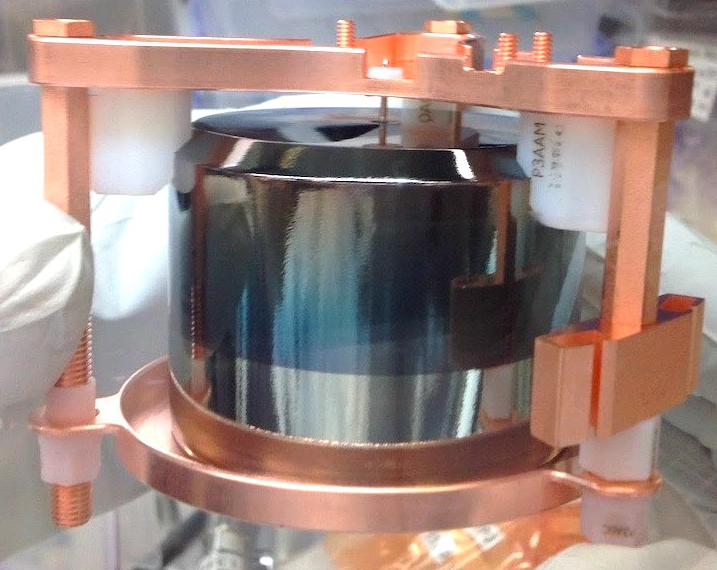
\includegraphics[height=6cm]{ortecdetector}}
  \caption[Natural and enriched detector photos]{\label{fig:detphotos}
    A photo of a natural detector with the BEGe geometry and an enriched detector. Note the LMFE electronics on top of the natural detector. The point contact, with copper pin inserted, is visible at the top of the enriched detector.
  }
\end{figure}
Two types of PPC detectors are used for the \MJD.
Many of the detectors use germanium with the natural isotopic abundance (7.8\% \Ge{76}), manufactured by CANBERRA using the Broad Energy Germanium (BEGe) detector geometry, and referred to as natural detectors.
The remaining detectors use Germanium that has been isotopically enriched to $88.1\pm0.7\%$ in \Ge{76}, manufactured by AMETEK/Ortec using a detector geometry with greater volume to surface area ratio than the BEGe detectors, and are referred to as enriched detectors.
Photographs of both an enriched and natural detector are shown in fiture~\ref{fig:detphotos}.
By isotopically enriching the germanium used to manufacture the detectors, they act as both the source and the detector of \znbb, with the result that all kinetic energy from a \znbb\ is detected, which ensures a high detection efficiency.
Furthermore, the manufacturing processes for HPGe detectors require a high material purity, which ensures intrisically low backgrounds inside of the detectors.

\begin{figure}[h]
  \centering
  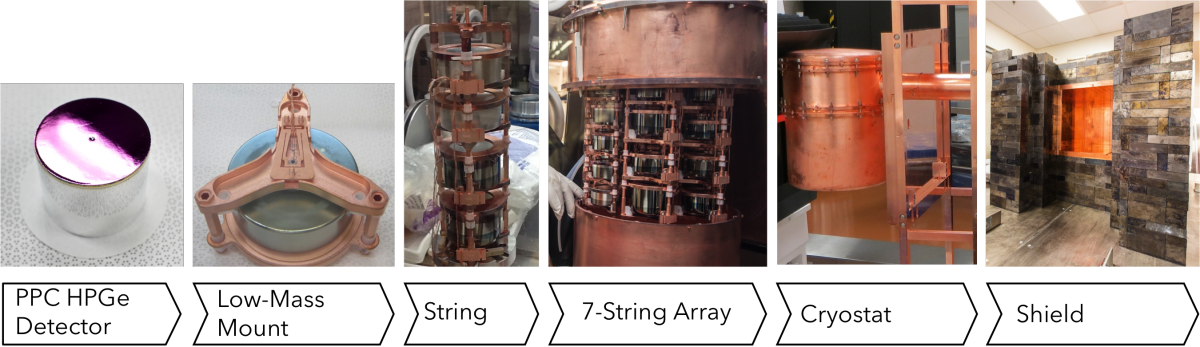
\includegraphics[width=\textwidth]{Modular_Design}
  \caption[Modular design of the \MJD]{\label{fig:modulardesign}
    Each stage in the staged design of the \MJD, from a detector to a module. Photos taken by Matt Kapust (SURF).
  }
\end{figure}
Because a single HPGe detector has a mass of $\sim0.5-1.1$~kg, in order to collect a high exposure, we build an array of detectors.
This has the further advantage that the detectors in the array help shield one another, resulting in lower backgrounds as the size of the array increases.
The \MJD\ used a staged, modular construction approach that is designed to be scalable towards a tonne-scale \znbb\ search.
Each detector is placed in interchangable detector mounts, to which the first stage preamplifier and signal and high voltage electronics cables are attached.
These mounts are stacked into strings of 4-5 detectors, which are arranged into arrays of 7 strings, and the arrays are placed into cryostats.
The detectors, electronics, cooling and vacuum  hardware are operated independantly for each cryostat, and the combination of this hardware and the detector array is refered to as a module.
Figure~\ref{fig:modulardesign} shows the various stages of a module.

\begin{figure}[h]
  \centering
  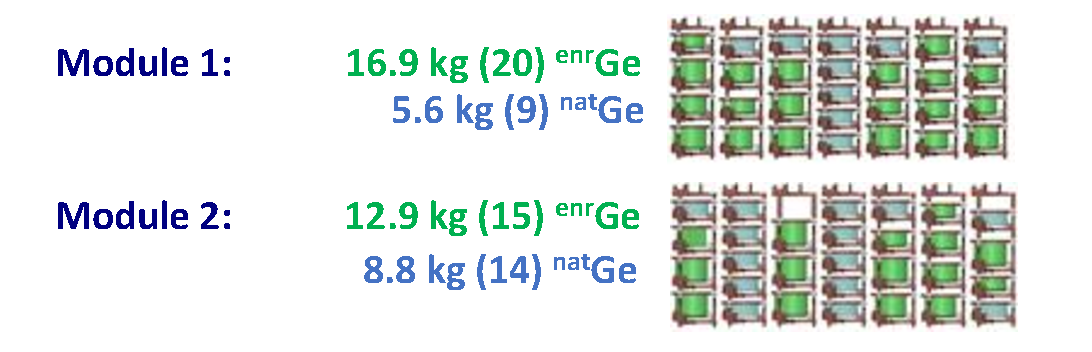
\includegraphics[width=0.9\textwidth]{modules}
  \caption[Layout of all strings in both modules with natural and enriched detectors labelled]{ \label{fig:modules}
    Layout of all strings in both modules. The center string for each module is furthest to the left, and the other strings are on the outside. Enriched detectors are colored green, and natural detectors are colored blue.
  }
\end{figure}
The \MJD\ has been constructed with two modules, shown in Figure~\ref{fig:modules}.
Module~1 contains 20~enriched detectors, totalling 16.9~kg in mass, and 9~natural detectors, totalling 5.6~kg.
Module~2 contains 15~enriched detectors, totalling 12.9~kg, and 14~natural detectors, totalling 8.8~kg.
In total, the total mass of \Ge{76} is 27.4~kg, 26.3~kg of which is contained in the enriched detectors.

To meet the stringent background requirements of the \MJD, the detector and cryostat components are built out of extra clean materials.
The cryostat and detector mount structures are built out of copper that has been electroformed underground\cite{mjdeforming}.
Insulating components consist of NXT-85, a low background Teflon.
The first stage preamplifier electronics, called Low Mass Front End (LMFE) boards, are mounted directly on top of the detector mounts, and are specially designed to minimize the amount of material required.
The high voltage and signal cables are manufactured by Axon' to minimize the component mass, and both use specially designed low mass, low background electrical connectors\cite{mjdHV, mjdsig}.
Exposure to the surface, where a high cosmic ray flux can cosmogenically activate radioactive isotopes such as \Co{60}, is minimized and tracked for all components, particularly the detectors and copper components\cite{mjdptdb}.
Components are machined underground in a class 1000 clean room environment, and kept in nitrogen purged environments as much as possible in order to avoid exposure to Radon.
\begin{figure}
  \centering
  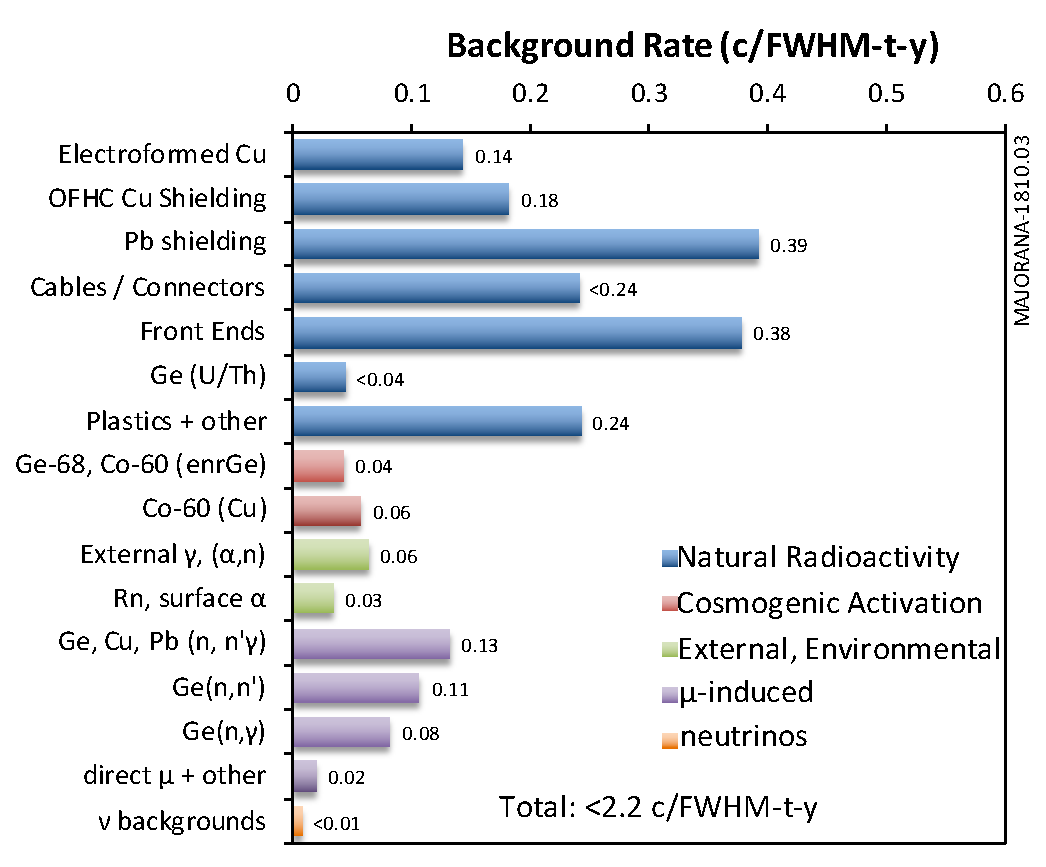
\includegraphics[width=0.6\textwidth]{bgassay}
  \caption[Background predictions based on component assays]{\label{fig:assay}
    Prediction of contribution to backgrounds in the ROI around 2039~keV from different sources, based on component assays and simulations.
  }
\end{figure}
An extensive radioassay campaign was carried out to verify the low backgrounds of the components and the manufacturing procedures\cite{mjdassay}.
The results of this assay campaign are shown in Figure~\ref{fig:assay}, and predict a background index of $<2.2$~cts/FWHM-t-y, with primordial isotopes in the LMFE boards and the lead shield as the dominant background contributions.

Each cryostat is placed inside of a graded shield in order to further reduce backgrounds.
Each layer of the shield is constructed from successiveley cleaner materials in order, consisting from outer- to inner-most layer of:
\begin{itemize}
\item High density polyethylene panels that reduce the energy of incoming environmental neutrons, and borated polyethylene to capture the neutrons
\item Scintillating acrylic veto panels that act as an active muon veto, to be described in greater detail in Section~\ref{sec:muonveto}
\item A mostly-sealed aluminum box that is continuously purged with scrubbed nitrogen gas in order to purge the interior of radon gas
\item A 45~cm thick lead shield
\item A 5~cm thick shield manufactured from commercially available Oxygen-Free High thermal Conductivity (OHFC) copper
\item A 5~cm thick shield manufactured from underground electroformed copper that has not been exposed to surface cosmic ray flux
\end{itemize}
\begin{figure}
  \centering
  \subfloat[Crossectional Diagram]{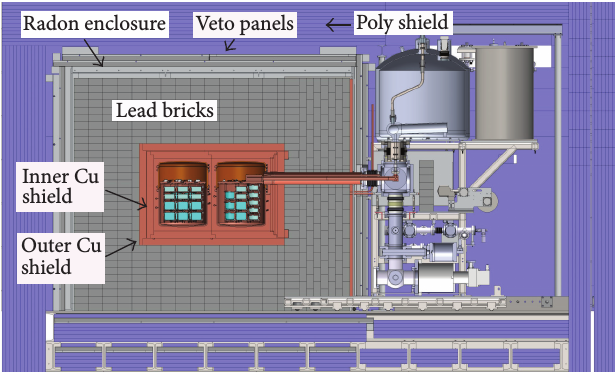
\includegraphics[width=\textwidth]{ShieldDiagram}}\\
  \subfloat[Lead Shield]{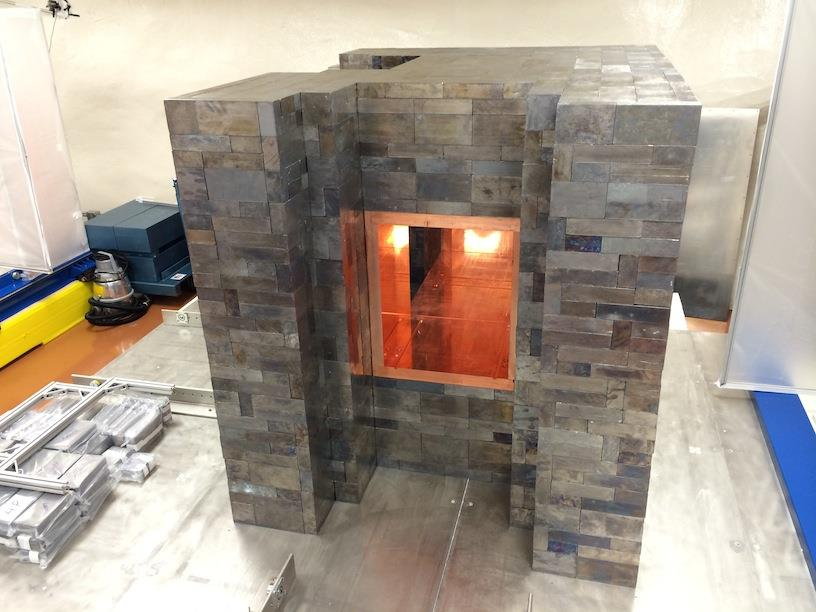
\includegraphics[width=0.45\textwidth]{leadshield}}~
  \subfloat[Overfloor]{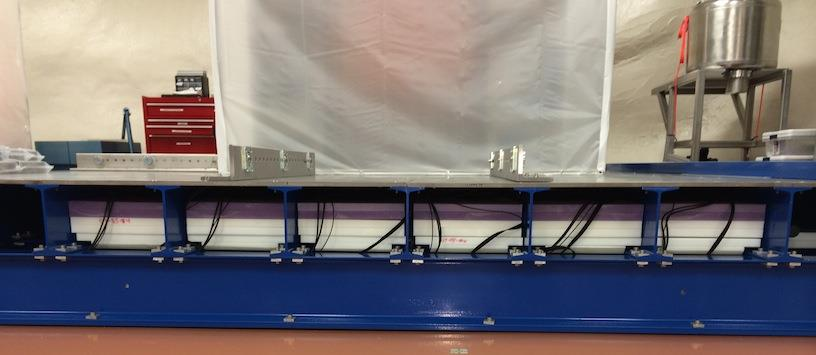
\includegraphics[width=0.5\textwidth]{overfloor}}
  \caption[Diagram of the \MJD\ shield]{\label{fig:shield}
    Top: A crossectional diagram showing the different layers of the shield. Bottom left: The lead shield and outer copper shield, prior to installation of other shield layers. Bottom right: The overfloor, atop which the shield is installed. The polyethylene and veto panels are visible.
  }
\end{figure}
Figure~\ref{fig:shield} contains a drawing of the shield and module hardware.
In addition to this shielding, the entire experiment is hosted at the Davis Campus of the Sanford Underground Research Facility (SURF) in Lead, South Dakota, 4850', with an overburden of $\sim4300$~m.w.e\cite{surf}.

\subsection{Muon Veto}\label{sec:muonveto}
The muon veto consists of 32~scintillating acryllic panels instrumented with wavelength-shifting fibers and photo-multiplier tubes \cite{2015wiseman}.
The panels are arranged to completely cover each face of the shielding, including the top and bottom, forming a completely enclosed surface.
As a result, any muon that passes through the \MJD\ shield system must cross at least 2~veto panels on at least 2~different surfaces of the shield, depositing on the order of several MeV in each one.
Furthermore, each surface has two orthogonal layers of panels, enabling a more precise reconstruction of the muon direction.
Figure~\ref{fig:muonveto} shows a diagram of the panel layout.
The muon veto is read out by two Caen QDC digitizers, with a separate Caen trigger card that acts as a 100~MHz clock and facilitates the trigger logic for the veto system.
All channels on all three cards are simultaneously recorded if any two panels simultaneously record energies greater than a threshold set a the hardware level.
LED pulsers are used to monitor the stability of each channel.

\begin{figure}
  \centering
  \subfloat[Muon veto panel configuration]{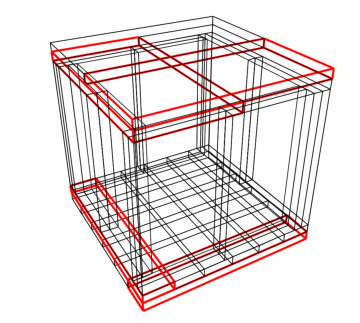
\includegraphics[width=0.4\textwidth]{muonpanels}}
  \subfloat[Muon induced events]{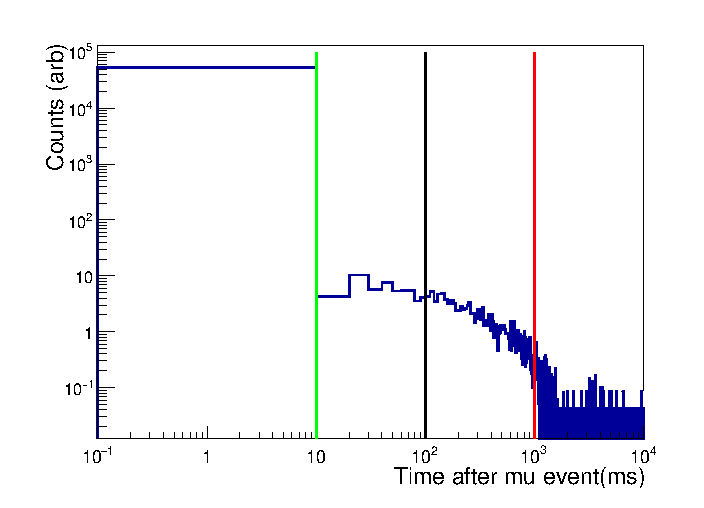
\includegraphics[width=0.6\textwidth]{muvetotiming}}
  \caption[Muon veto system]{\label{fig:muonveto}
    Left: the muon veto panel configuration. An example of a muon hit pattern is shown using the red-highlighted panels.\\
    Right: a simulation of the timing distribution of HPGe events induced by muons, relative to the muon timing. The timing cutoff is shown using the red line.
  }
\end{figure}
Each muon event is analyzed to identify candidate muons.
LED pulsers, which affect all panels simultaneously, $\gamma$-rays, which will have lower energies and different hit patterns, and events caused by hardware errors can be easily identified and removed.
This analysis is expected to tag $>99\%$ of muon events that pass through the shield, with exceptions during DS0 and DS1, prior to the completion and complete debugging of the veto system.
Once muon events have been analyzed, any HPGe detector events in a range of 0.2~ms before 1~s after the event are cut.
As shown in Figure~\ref{fig:muonveto}, this cut is expected to remove $>99.9\%$ of events induced by through-going muons, with exceptions during DS0 and DS1 when the muon and HPGe detector clocks were desynchronized.
In addition to acting as a veto, this system can produce analyses of the muon flux measured at SURF's Davis Campus\cite{mjdmuonflux}.

\section{HPGe Detector Signal Processing} \label{sec:mjprocessing}
This section will describe how a signal from one of the \MJD's detectors is read out, starting with the detector electronics, through the digital waveform processing techniques that are used.

\subsection{Charge Signal Collection} \label{sec:signalelectronics}
\begin{figure}
  \centering
  \subfloat[Circuit Diagram]{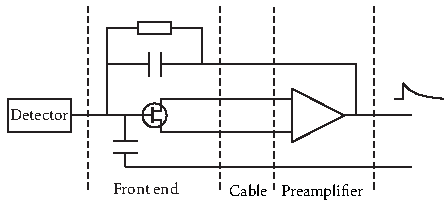
\includegraphics[width=.55\textwidth]{lmfediagram}}
  ~\subfloat[LMFE Board]{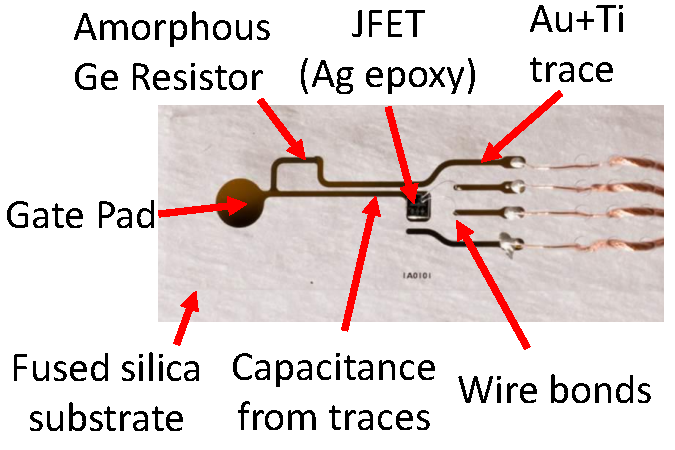
\includegraphics[width=.4\textwidth]{lmfephoto}}
  \caption[LMFE circuit diagram and photo]{\label{fig:lmfe}
    A circuit diagram and labelled photo of an LMFE board. The convergence of the traces on the board act as a charge-integrating capacitor.
  }
\end{figure}
When an event occurs inside of a PPC HPGe detector, a cloud of free conduction band electrons and positively charged valance band vacancies called holes is produced.
Under the influence of a high voltage applied across the detector (1-5~kV), the electrons drift towards the $n^+$ contact and the holes towards the $p^+$ contact, inducing a charge signal at the $p^+$ contact.
The total charge produced is proportional to the energy of the event, with one electron-hole pair produced for every 0.7~eV of energy deposited.
The induced charge signal is measured by the LMFE board, which is a charge sensitive preamplifier that is resistively coupled to ground\cite{barton2012}.
The LMFE is mounted directly on each detector mount, offset by $<1$~cm, in order to minimize electronics noise and crosstalk between electronics channels.
The LMFE is connected by electronic cables to a second stage amplifier outside of the lead shield.
The second stage amplifier produces two separate signals, with differing gains; the low gain channel saturates at higher energies, while the high gain channel has better noise characteristics at lower energies.
For the analysis presented here, events from the high gain channel will be primarily used.
This circuit results in a typical peakshape that is approximately exponential, with a tail of $\sim72~\mu$s.
The LMFE board additionally has a capacitively-coupled pulser line that can produce artificial pulses of a fixed energy that can be used to monitor the stability of the electronics.
A circuit diagram and photo for the LMFE board is shown in Figure~\ref{fig:lmfe}.
A waveform shaped by these electronics can be seen in Figure~\ref{fig:trapfilter}.

For each detector, the signal from both channels is digitized using GRETINA digitizer cards, developed by the GRETINA experiment\cite{zimmermann2012}.
The \MJD\ signals are digitized at a freqency of 100~MHz, with 14 bits of precision.
A built in field-programmable gate array applies a pole-zero correction and trapezoidal filter independantly to each channel (these will be discussed in the next section).
Each channel is independantly triggered using a leading edge discrimination on the trap-filtered waveform, and records 2020 samples per waveform.
The digitizers are further capable of presumming samples by factors of 2, 4, 8 or 16, enabling variable length traces.
Furthermore, the ditizizers can multi-sample, using a different presumming factor for different portions of the waveform.
Multi-sampling enables a high sampling frequency for the rising edge of the waveform, which aids the PSA techniques that depend on the waveform risetime, and a low sampling frequency for the falling tail and baseline of the waveforms, which improves baseline measurement, energy estimation, and PSA techniques that utilize the exponential tail of the waveform.
For \MJD\ data, for different datasets, multi-sampling is either disabled, resulting in $\sim20~\mu$s waveforms with a single sampling frequency of 100~MHz, or enabled with the falling tail sampled at 25~MHz, resulting in $\sim40~\mu$s waveforms.
Each digitized pulse is recorded and reanalyzed offline, using the software described in Section~\ref{sec:mjsw}.

\subsection{Energy Estimation}
\begin{figure}
  \centering
  \subfloat[Raw Waveform]{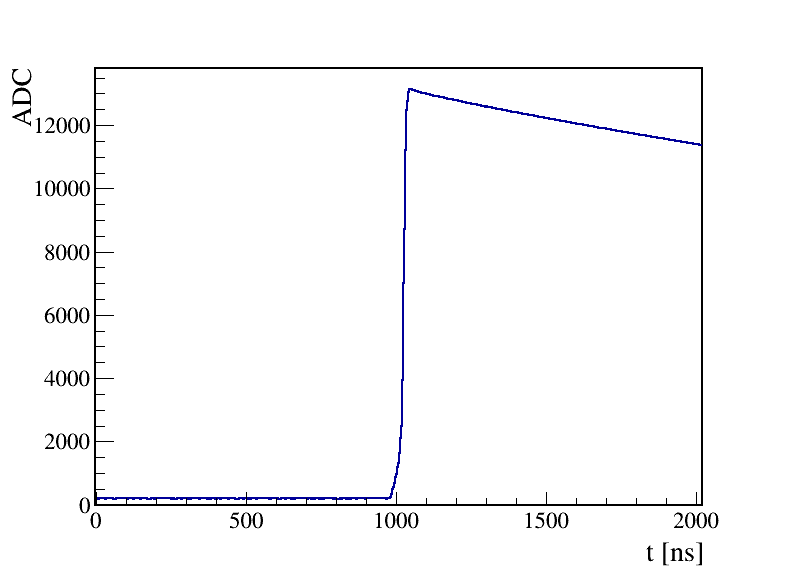
\includegraphics[width=.33\textwidth]{rawWF}}
  \subfloat[Pole-zero Correction]{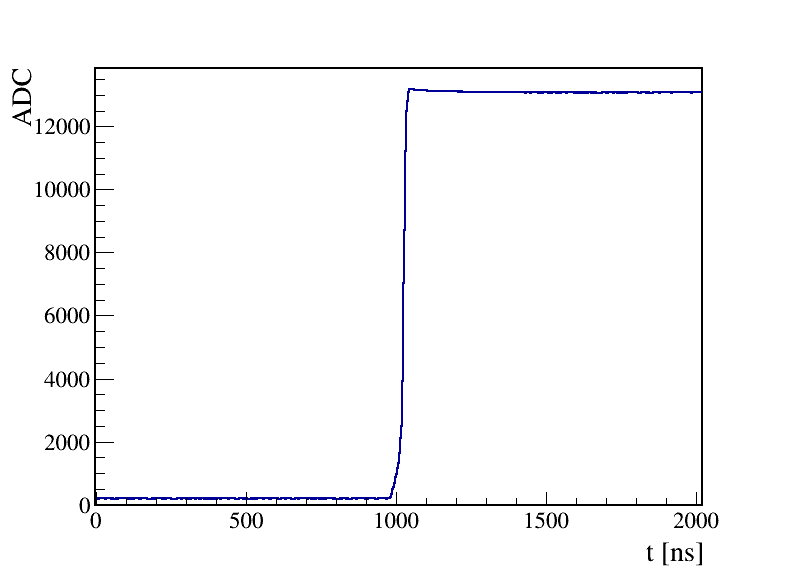
\includegraphics[width=.33\textwidth]{PZWF}}
  \subfloat[Trapezoidal Filter]{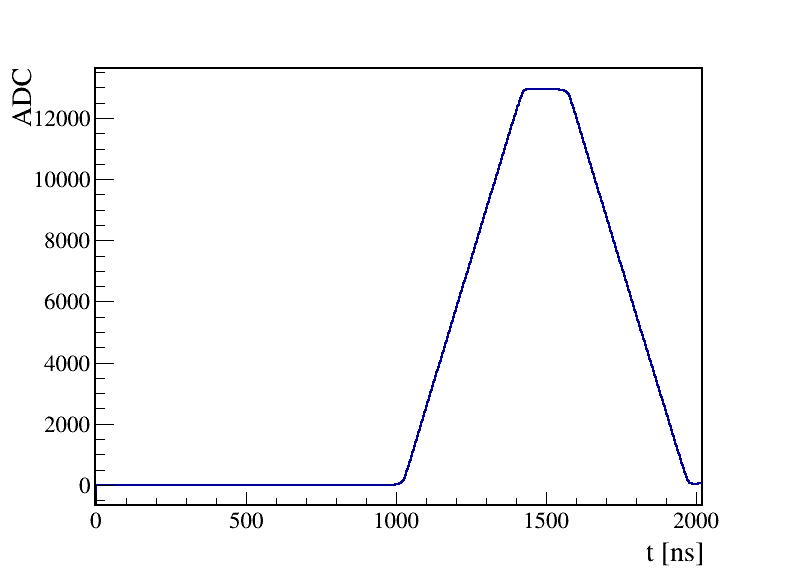
\includegraphics[width=.33\textwidth]{trapWF}}
  \caption[Pole-zero correction and trapezoidal filter]{\label{fig:trapfilter}
    Left: A raw waveform as shaped by the signal electronics, with a time constant of $\sim72~\mu$s\\
    Center: the same waveform after pole-zero correction, with a (nearly) flat top
    Right: the same waveform after application of a trapezoidal filter
  }
\end{figure}
The energy of a waveform is estimated using a trapezoidal filter implemented in software.
Trapezoidal filters are nearly optimal filters for energy estimation, enabling low noise measurements while avoiding ballistic deficit\cite{Radeka1972, knoll}.
The trapezoidal filter has a flat top length of $2~\mu$s and a ramp-time of $4~\mu$s.
The pole-zero constant is optimized independantly for each detector in order to produce a flat-top for the trapezoids, and the maximum value of the trapezoid is selected as the energy estimator.
An example of a pole-zero correction and trapezoidal filter application is shown in Figure~\ref{fig:trapfilter}.
The energy measured in this fashion is named \texttt{trapENF}.

\subsection{Additional Energy Corrections} \label{sec:energy}
\begin{figure}
  \centering
  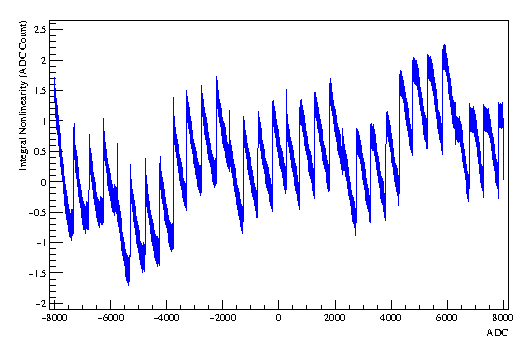
\includegraphics[width=0.6\textwidth]{dignonlin}
  \caption[Integral digitizer nonlinearity]{\label{fig:localnonlin}
    The shift in the value of each ADC bin that is applied in order to achieve a linear digitizer response with respect to voltage. This is measured by integrating over the width of each ADC bin, and is referred to as Integral nonlinearity.
  }
\end{figure}
A second energy estimator has been implemented that corrects for several systematic errors in the \texttt{trapENF} estimator\cite{energyunidoc}.
First, nonlinearities in the digitizer response are corrected for.
The GRETINA digitizers have an unusually large nonlinearity, which manifests as a periodic sawtooth-shaped error, as shown in Figure~\ref{fig:localnonlin}.
The size of this nonlinearity is measured by applying external, ramping signals from waveform generators in order to measure the width of each ADC bin.
The resulting size of this nonlinearity before correction can shift measured energies by as much as 0.8~keV in the high gain readout.
Before applying a trapezoidal filter, each waveform sample is corrected by the measured integral nonlinearity value, reducing the size of the ADC nonlinearity to $<0.1$~keV.
The residual nonlinearity in energy response after applying this correction is referred to as the local nonlinearity.

\begin{figure}
  \centering
  \subfloat[Modified Pole-Zero]{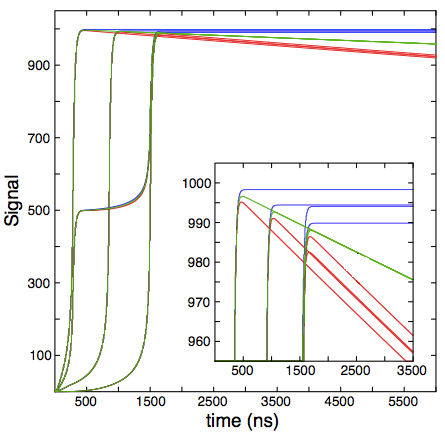
\includegraphics[height=6cm]{ctcorrection}}
  \subfloat[FWHM Optimization]{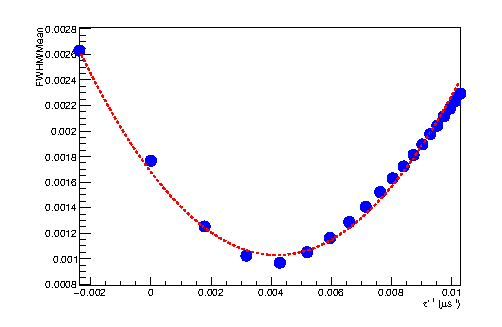
\includegraphics[height=6.4cm]{fwhmoptimization}}
  \caption[Charge Trapping Correction]{\label{fig:ctcorr}
    On the left, three waveforms are shown with different pole-zero constants applied. For the flat top pole-zero constant (blue), the tops are misalligned due to a loss of charge from charge trapping. For the charge trapping corrected pole zero constant (green), the tops are no longer flat, but they align perfectly, resulting in improved energy resolution. On the right, we see the FWHM of a 2614~keV $\gamma$ peak as a function of the pole-zero constant. By optimizing the FWHM, we can identify the correct time constant to use for the charge trapping correction. 
  }
\end{figure}
A second correction is applied to correct for charge trapping.
Charge trapping is a phenomenon in which local impurities in a HPGe detector capture electrons or holes as they drift to the $n^+$ and $p^+$ contacts, respectively.
This results in a loss of charge collection that is dependant on the origin location of the charge cloud within the detector.
This charge loss distorts the detector response, producing a low-energy tail in the peak shape, and degrades the energy resolution.
The resolution degradation increases linearly as a function of hit energy, and at energies near the Q-value, this is a dominant contribution to the peak width.
Charge trapping can be modelled as an exponential loss of charge with respect to the drift time of the charge inside of the HPGe crystal.
To correct for this, we modify the pole-zero time constant so that the flat-top of the trapezoidal filter decays with the same time-constant as the charge trapping.
As a result of this change, the measured waveform response after full charge collection will be identical, with respect to the origin time of the charge cloud, as shown in Figure~\ref{fig:ctcorr}.
The resulting pole-zero time $\tau$ is described by:
\begin{equation}
  \frac{1}{\tau} = \frac{1}{\tau_{PZ}} + \frac{1}{\tau_{CT}}
\end{equation}
where $\tau_{PZ}$ is the flat-top pole-zero time constant, and $\tau_{CT}$ is the charge trapping time constant.
The value of $\tau$ is chosen to optimize the FWHM measured for a 2614~keV peak from a \Th{228} calibration spectrum, using the energy estimator described here.
This optimization is shown in Figure~\ref{fig:ctcorr}.

\begin{figure}
  \centering
  \subfloat[\texttt{trapE} vs \texttt{trapENF}]{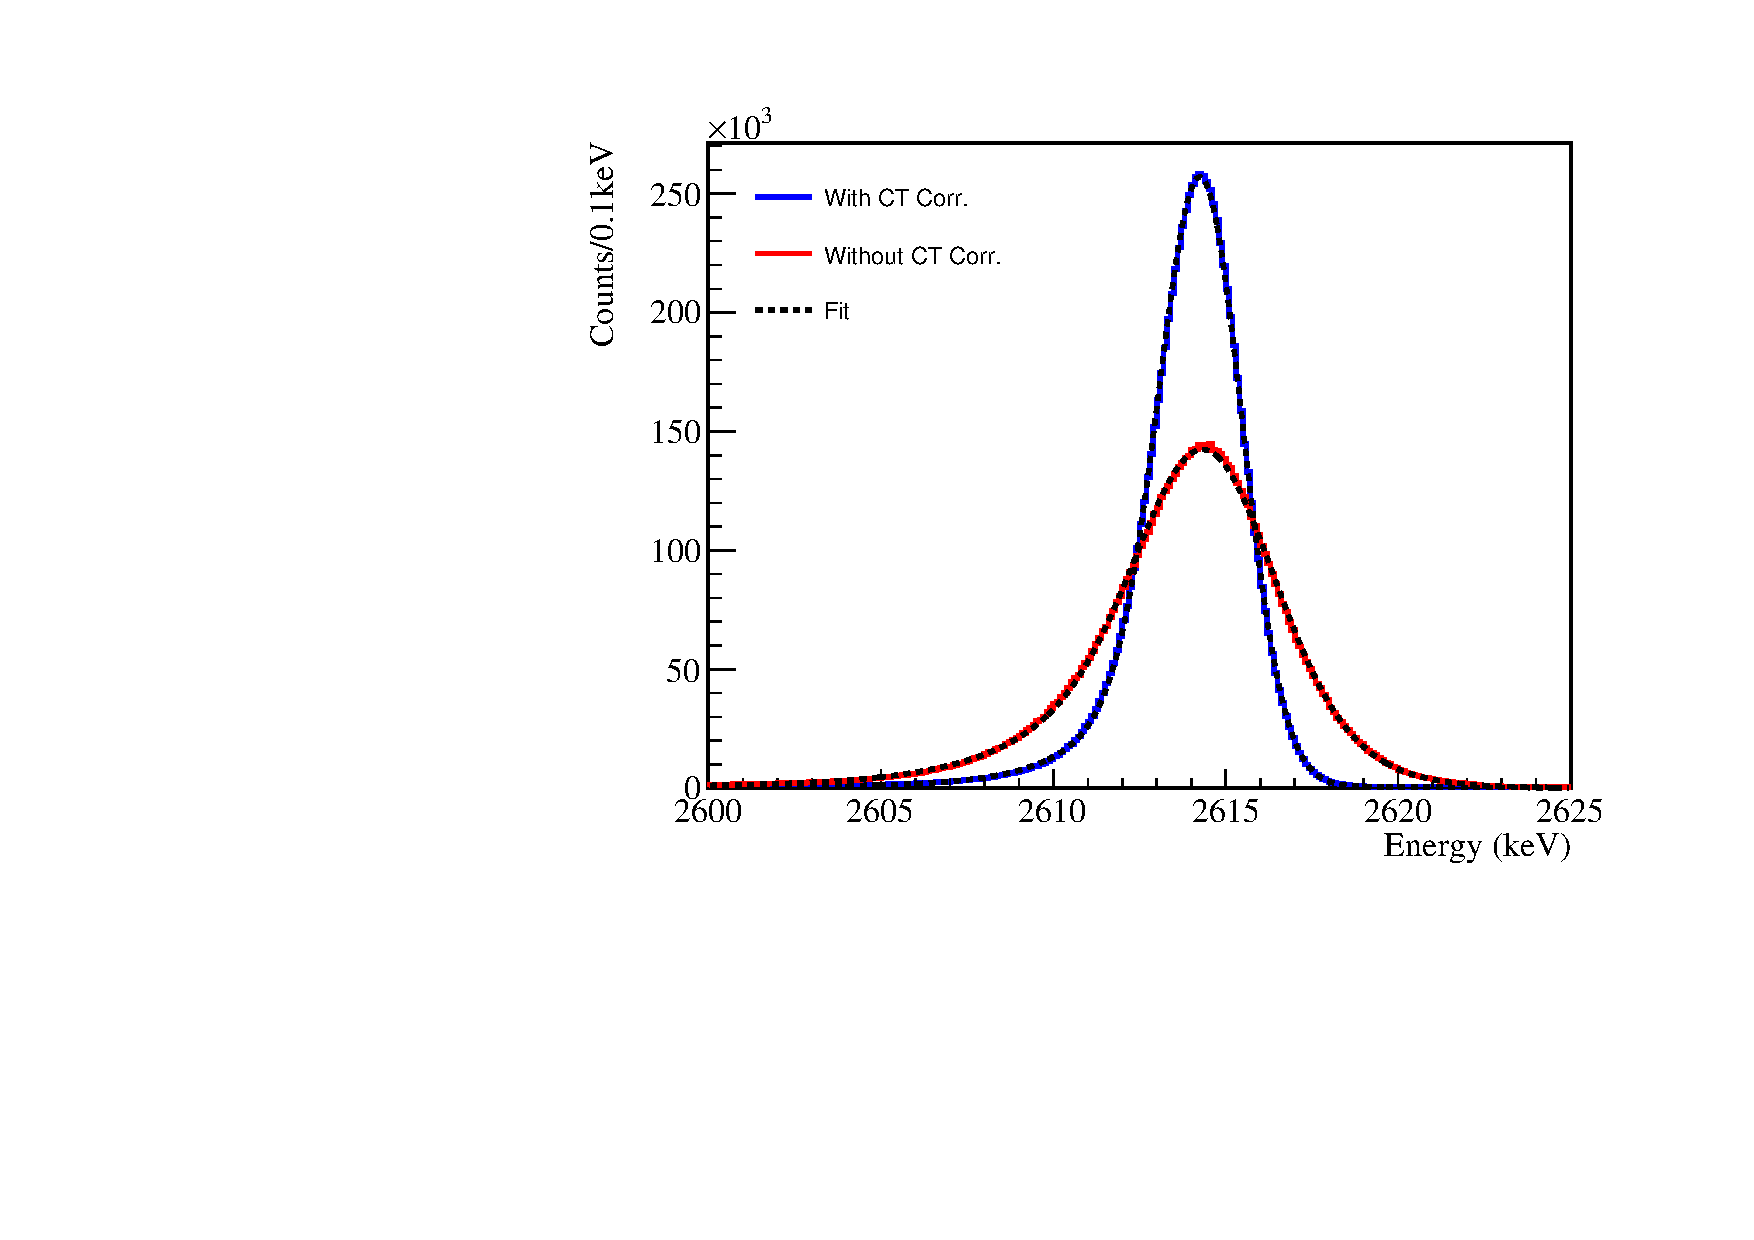
\includegraphics[width=0.53\textwidth]{trapEvtrapENF}}
  \subfloat[Improvement in Energy Resolution]{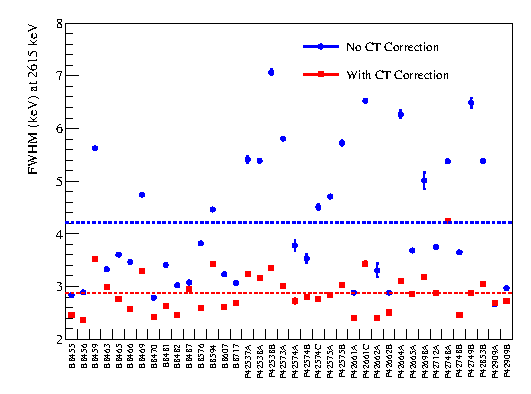
\includegraphics[width=0.47\textwidth]{ctimprovement}}
  \caption[Improvement in energy resolution from charge trapping correction]{\label{fig:trapenf}
    The energy resolution is improved as a result of applying the charge trapping and digitizer nonlinearity corrections in a $\sim31\%$ improvement in energy resolution on average.
  }
\end{figure}
However, because the trapezoid no longer has a flat top, the maximum value is no longer useful as an energy estimator; instead, the amplitude of the trapezoid at a fixed time relative to the origin time of the trapezoid is used.
This technique is referred to as a ``fixed-time pickoff.''
A short trapezoidal filter with a rise-time of $1~\mu$s and a flat-top of $1.5~\mu$s is used, with the final crossing of a fixed threshold value used to estimate the origin time.
After applying both of these corrections, the resulting energy estimator is called \texttt{trapENF}.
The \texttt{trapENF} estimator improves the energy resolution of the \MJD\ detectors at 2614~keV by $\sim31\%$, as shown in Figure~\ref{fig:trapenf}.
Using the \texttt{trapENF} energy estimator, the \MJD\ has achieved the best energy resolution of any current generation \znbb\ experiment.
There is, however, still room for improvement by correcting for global nonlinearities that arise from an energy dependant, systematic drift in the start time estimator and a small quadratic nonlinearity in the detector response.

\subsection{Energy Calibration} \label{sec:calibration}
\begin{figure}
  \centering
  \subfloat[Calibration track drawing]{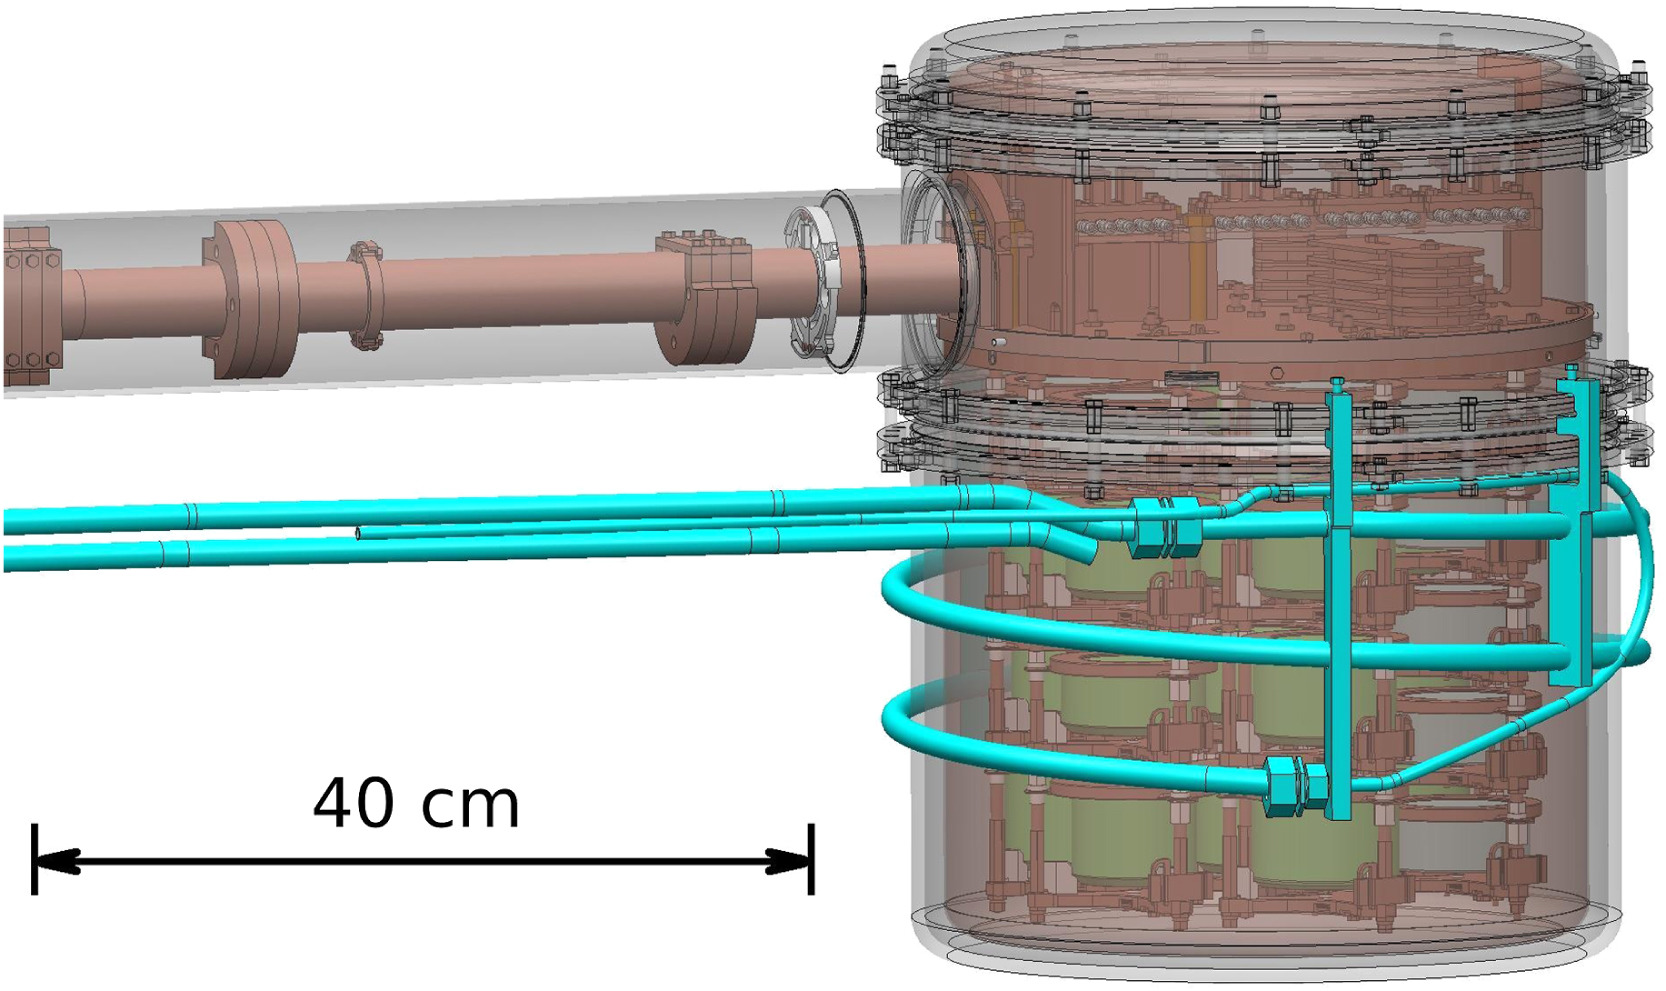
\includegraphics[width=0.45\textwidth]{calibrationtrackdrawing}}~
  \subfloat[Calibration track photo]{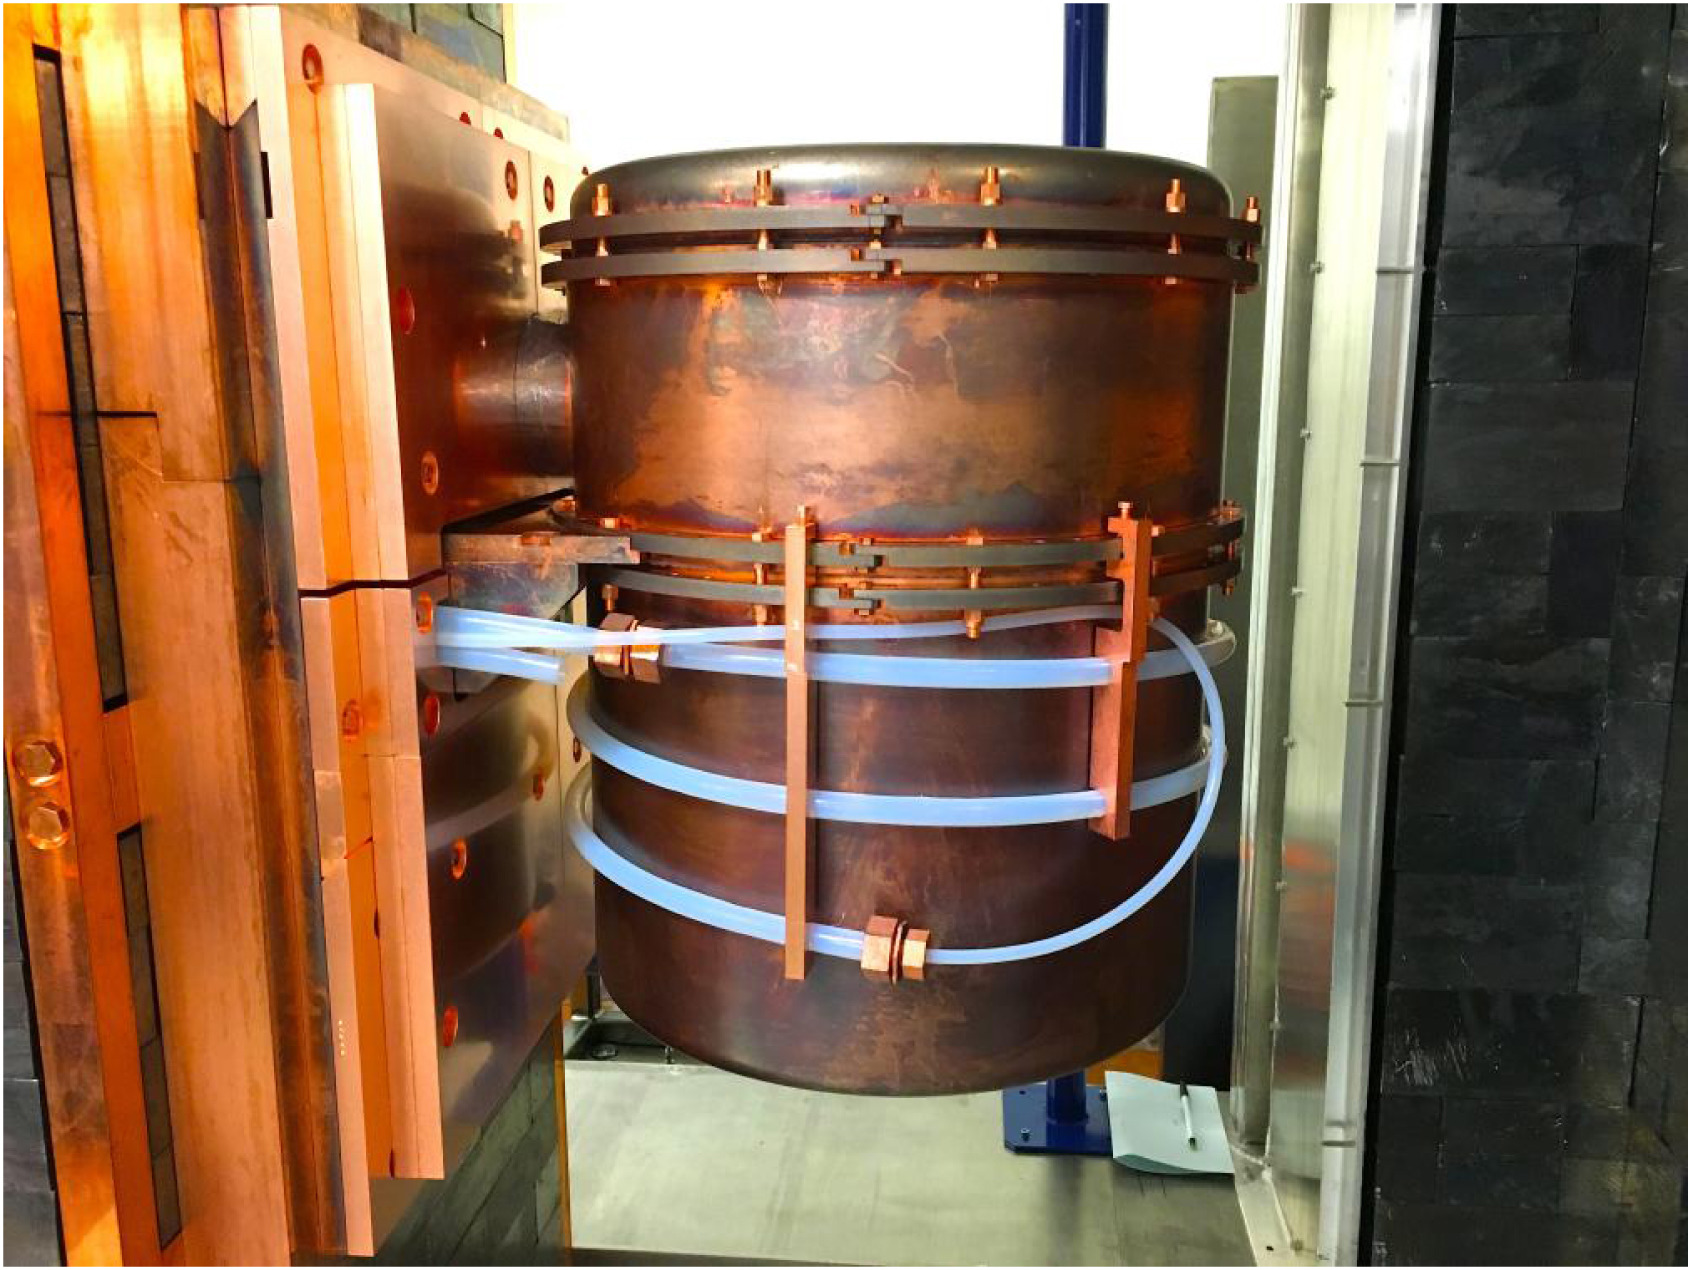
\includegraphics[width=0.45\textwidth]{calibrationtrackphoto}}
  \caption[Calibration track]{\label{fig:caltrack}
    A drawing and photo of the teflon calibration track wrapping around a cryostat.
  }
\end{figure}
Energy calibration of detectors is performed using a \Th{228} source\cite{mjdcalibration}.
\Th{228} has a large number of prominent $\gamma$-rays in its decay chain between 238~keV and 2614~keV which can be used to calibrate and characterize the detectors.
For each module, a 4.7~m long line source, consisting of \Th{228} doped epoxy, is used to perform calibrations, with an activity of $\sim10$~kBq along the last 2~m of the source.
The line source is inserted into guide tubes that wrap around the cryostat and reach outside of the shield structure.
The source is pushed by a motor located outside of the shielding, and a set of magnets and magnetic sensors are used to ensure that the source is placed in the correct position.
For each module, a separate 90~minute calibration run is performed once per week, with one source inserted at a time.
In addition to the \Th{228} line source, a \Co{60} line source with activity 6.3~kBq over the last 2~m of length and a \Co{56} line source with activity 6~kBq over the last 2~m of length were manufactured for use inside of the calibration track.
Figure~\ref{fig:caltrack} shows a drawing and photograph of the calibration track.

\begin{figure}
  \centering
  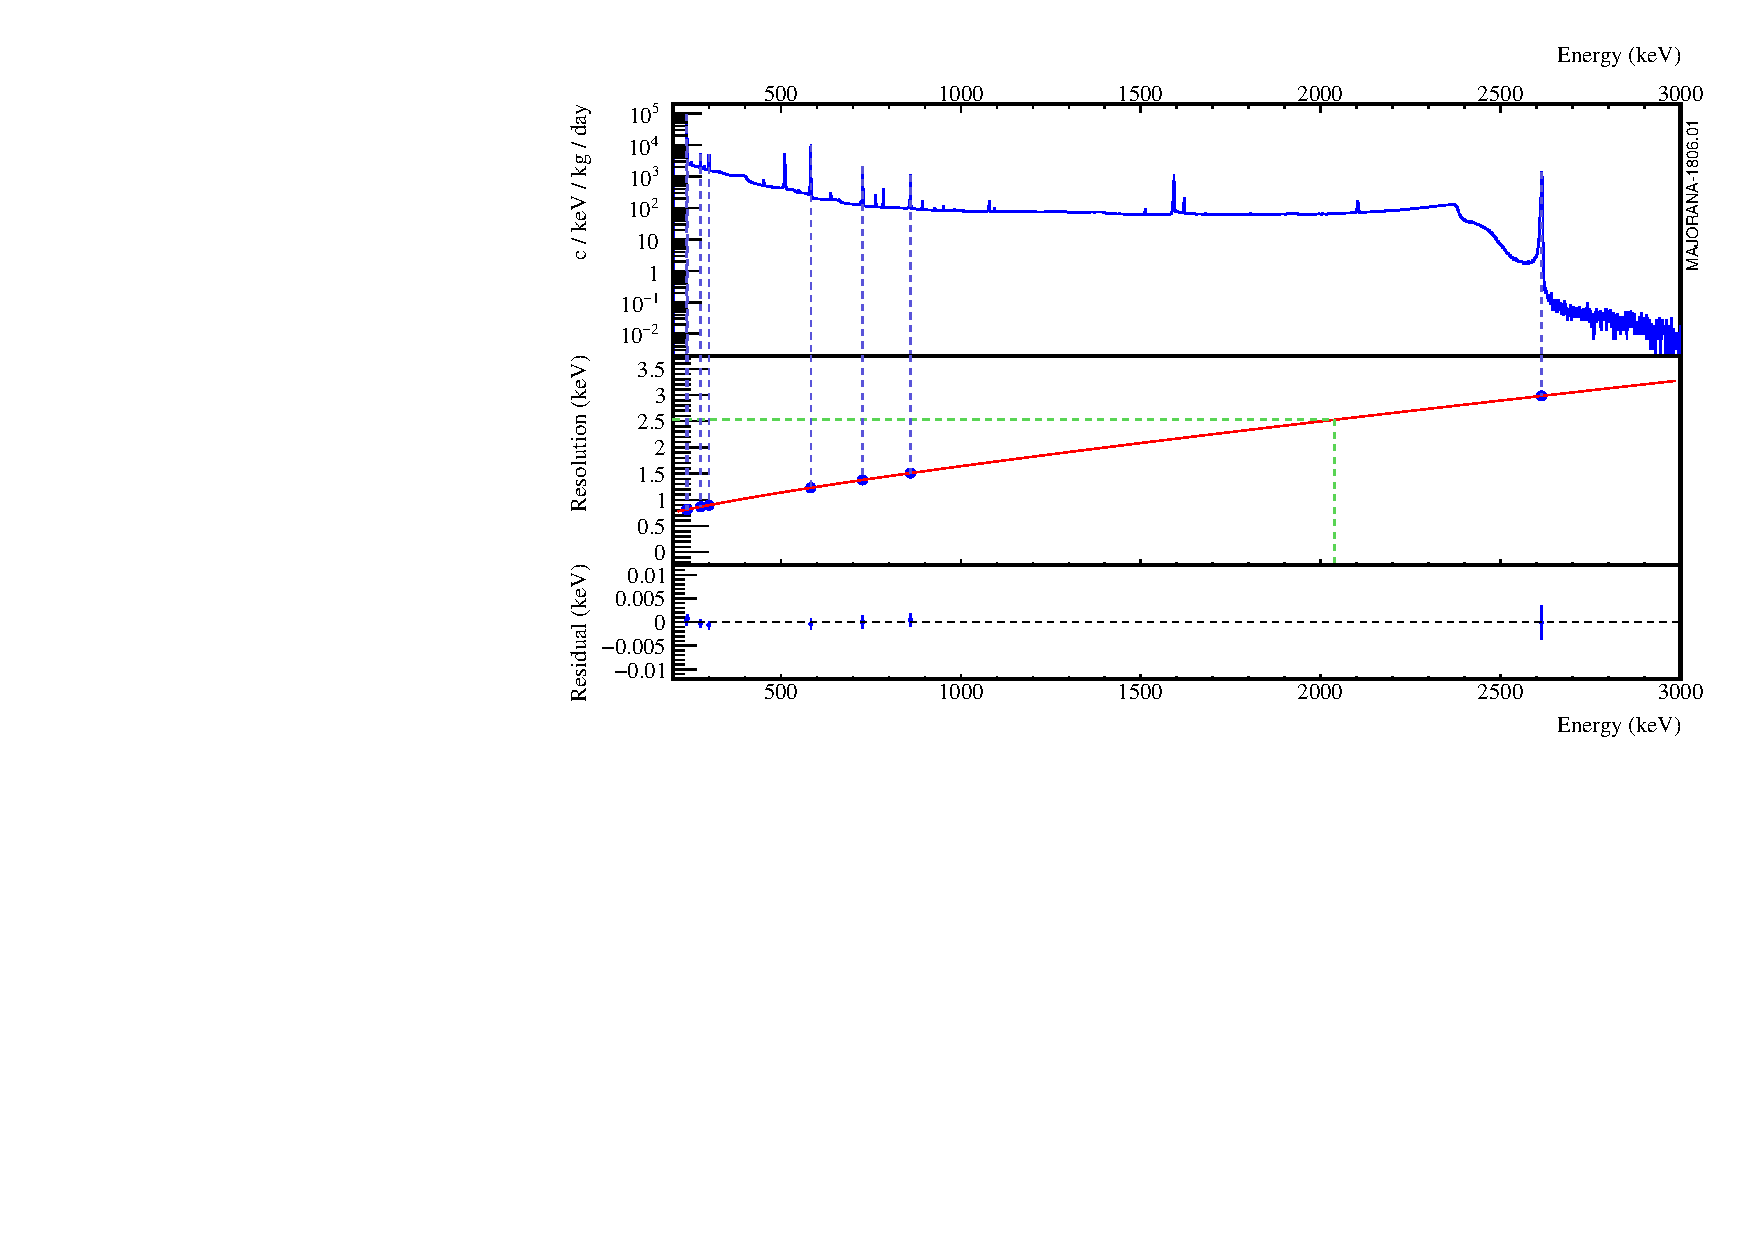
\includegraphics[width=\textwidth]{calfwhm}
  \caption[Calibration spectrum with FWHM]{\label{fig:calfwhm}
    A combined detector spectrum from a \Th{228} calibration run, with the FWHM extracted from a simultaneous fit of many peaks.
  }
\end{figure}
The $\gamma$ peaks from the \Th{228} spectrum are simultaneously fit to an analytic peakshape function, as described in Appendix~\ref{app:peakshape}.
The results of this fit are used to extract the gain, energy offset, and energy resolution of each HPGe detector, and of the combined detector array.
This fit is performed on 8~calibration peaks for each 90~minute calibration run, and a gain matching of the 238- and 2614-keV peaks is used to calibrate the detectors.
At the end of a major dataset, a more detailed fit of $\sim30$~peaks is performed, which is used to measure the detailed energy characteristics.
Figure~\ref{fig:calfwhm} shows a \Th{228} calibration spectrum, with the energy resolution extracted from a simultaneous peak fit.

\subsection{Multi-site Events} \label{sec:avse}
\begin{figure}[h]
  \centering
  \subfloat[PPC Field Map]{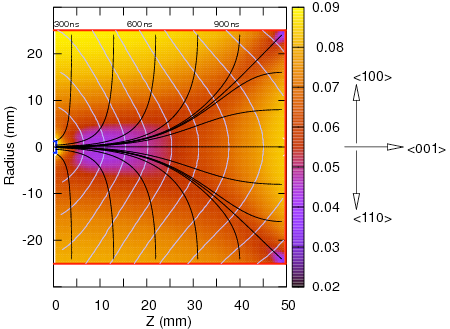
\includegraphics[width=0.5\textwidth]{ppcfieldmodel}}
  \subfloat[PPC Weighting Potential]{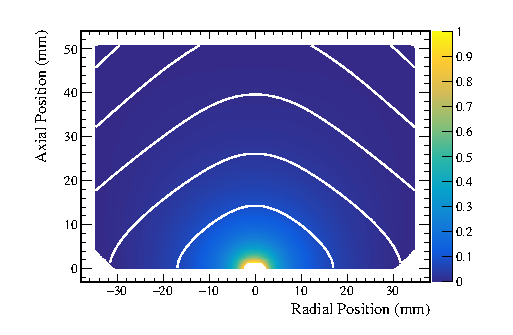
\includegraphics[width=0.5\textwidth]{ppcweightingpotential}}
  \caption[Electric field model of a PPC detector]{\label{fig:ppcdet}
    Left: a color map of the electric field strength in a PPC detector, with electron-hole drift paths (black) and surfaces of constant hole-drift time (grey).\\
    Right: a color map of the weighting potential in a PPC detector, which is highly localized near the point contact.
  }
\end{figure}
PPC HPGe detectors enable several PSA techniques that can differentiate between different types of events, which can aid in reducing backgrounds.
The PPC detector geometry results in low drift velocity in the bulk of the detector and a weighting potential that is highly locallized near the point contact, meaning that most of the charge signal is induced in a short period of time, as shown in Figure~\ref{fig:ppcdet}.
The result is a sharp current signal whose timing depends heavily on the position of charge deposition inside of the detector.
This enabled the discrimination of single-site events from multi-site events.
All charge in a single-site event is localized within $\sim1-2$~mm inside of the crystal.
$\beta\beta$-decay is an inherently single-site event because both electrons from the decay are fully absorbed within $\sim1$~mm of the decay site.
In multi-site events, multiple localized clusters of charge are simultaneously created in the crystal, separated by more than a few mm.
$\gamma$-rays that Compton scatter inside of the crystal and then deposit their remaining energy elsewhere in the crystal are an example of a multi-site event that could potentially be a background in searching for \znbb.
The charge drift times inside of PPC detectors is long enough that the drift time of each localized charge cloud in the detector will differ by potentially hundreds of ns, which is long enough to be visible to the GRETINA digitizers.
Figure~\ref{fig:avse} shows the difference between a single- and multi-site waveform.

\begin{figure}
  \centering
  \subfloat[Single- and Multi-site waveforms]{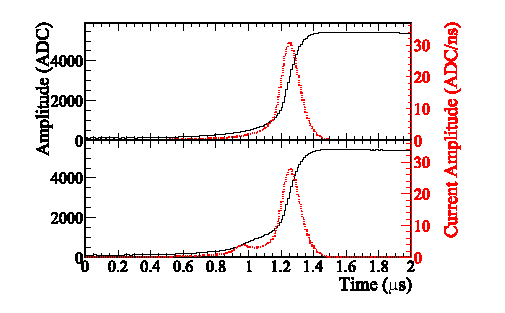
\includegraphics[width=0.5\textwidth]{ssmswf}}
  \subfloat[Calibration track photo]{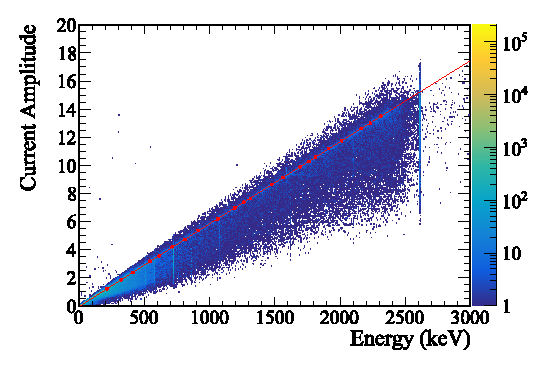
\includegraphics[width=0.5\textwidth]{avse}}
  \caption[Multi-site event cut]{\label{fig:avse}
    Left: A single-site event (top) and multi-site event (bottom). Note the multiple current pulses in the multi-site event, which results in a lower ratio of current amplitude to energy.\\
    Right: Comparison of current amplitude to energy. The red line represents the expected value for single-site waveforms. Waveforms that fall below the red line will mostly be multi-site waveforms. The AvsE parameter is calculated based on a comparison between the measured current amplitude, and the expected current amplitude for a singli-site event at that energy.
  }
\end{figure}
In order to distinguish between single- and multi-site waveforms, we compare the maximum current amplitude in the waveform to the total energy of the waveform\cite{mjdavse}.
For a single localized charge cloud, the maximum charge amplitude is expected to be approximately proportional to the energy deposited in the local area.
This means that single-site events will typically have a fixed ratio between these values.
In a multi-site event, on the other hand, the maximum charge amplitude will be proportional to the energy of the largest local site rather than the full energy of the waveform, so this ratio will be less than that for single-site events.
In Figure~\ref{fig:avse}, the relationship between the maximum current amplitude and the energy is shown.
The analysis parameter AvsE performs a comparison between these values and has been shown to cut $\sim95\%$ of multi-site events while keeping $\sim90\%$ of single-site events.
A measurement of these efficiencies is shown in figure\ref{fig:avseeff}
Near the \znbb\ region of interest, this cut removes $\sim60\%$ of Compton continuum backgrounds.
\begin{figure}
  \centering
  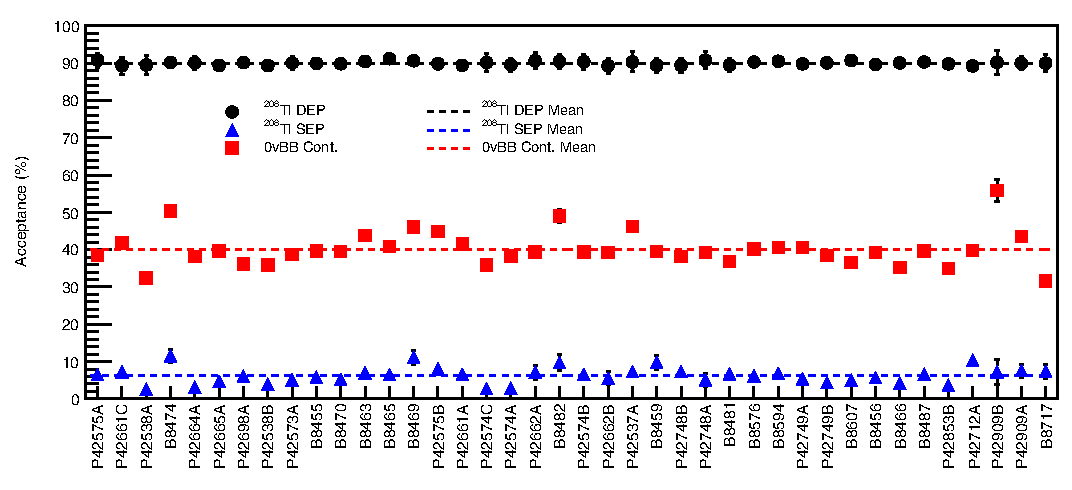
\includegraphics[width=\textwidth]{avseefficiency}
  \caption[Multi-site waveform cut efficiency]{\label{fig:avseeff}
    A measurement of the cut efficiency of the AvsE cut for single escape (SEP) events, which are inherently multi-site, double-escape (DEP) events, which are inherently single-site, and Compton continuum events.
  }
\end{figure}

\subsection{Surface Events} \label{sec:dcr}
\begin{figure}
  \centering
  \subfloat[DCR and Bulk Waveform]{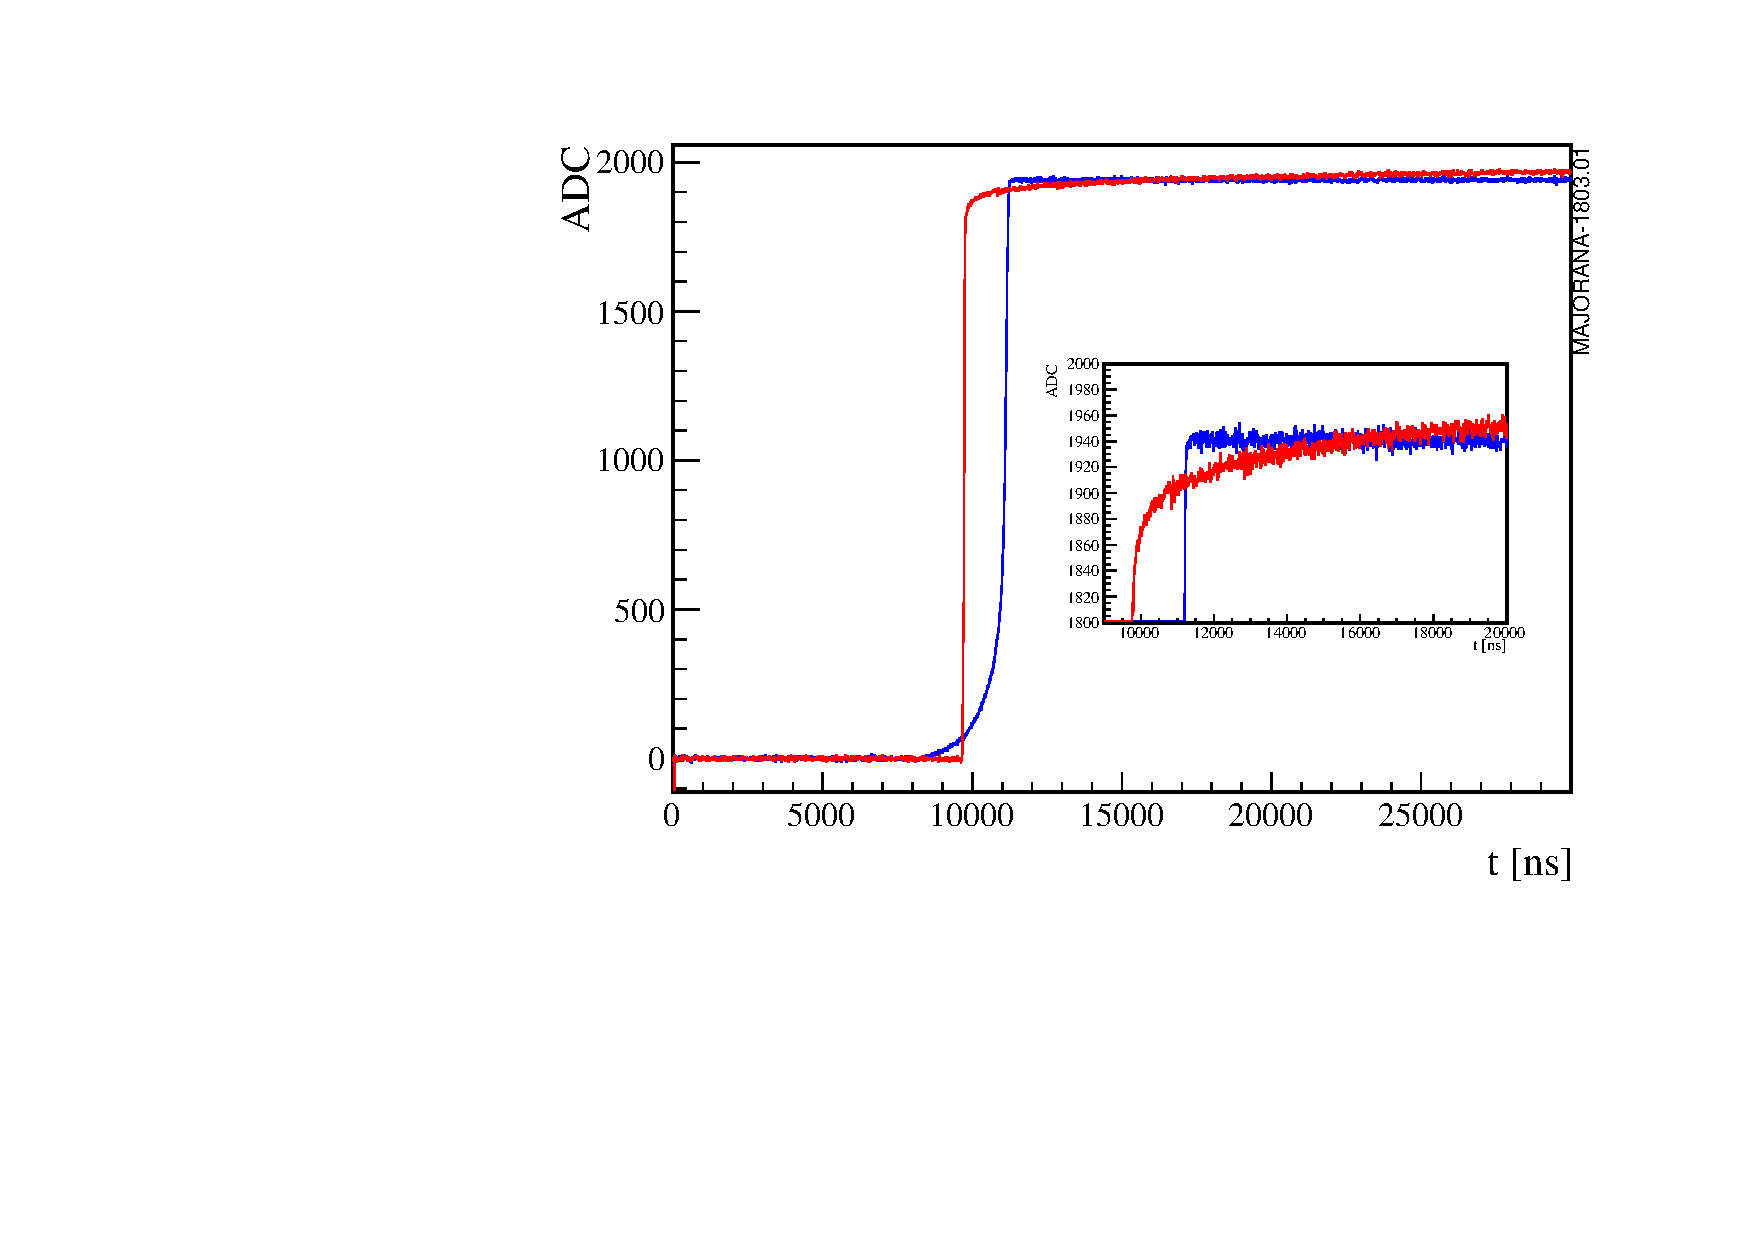
\includegraphics[width=0.46\textwidth]{DCRwf}}
  \subfloat[DCR distribution]{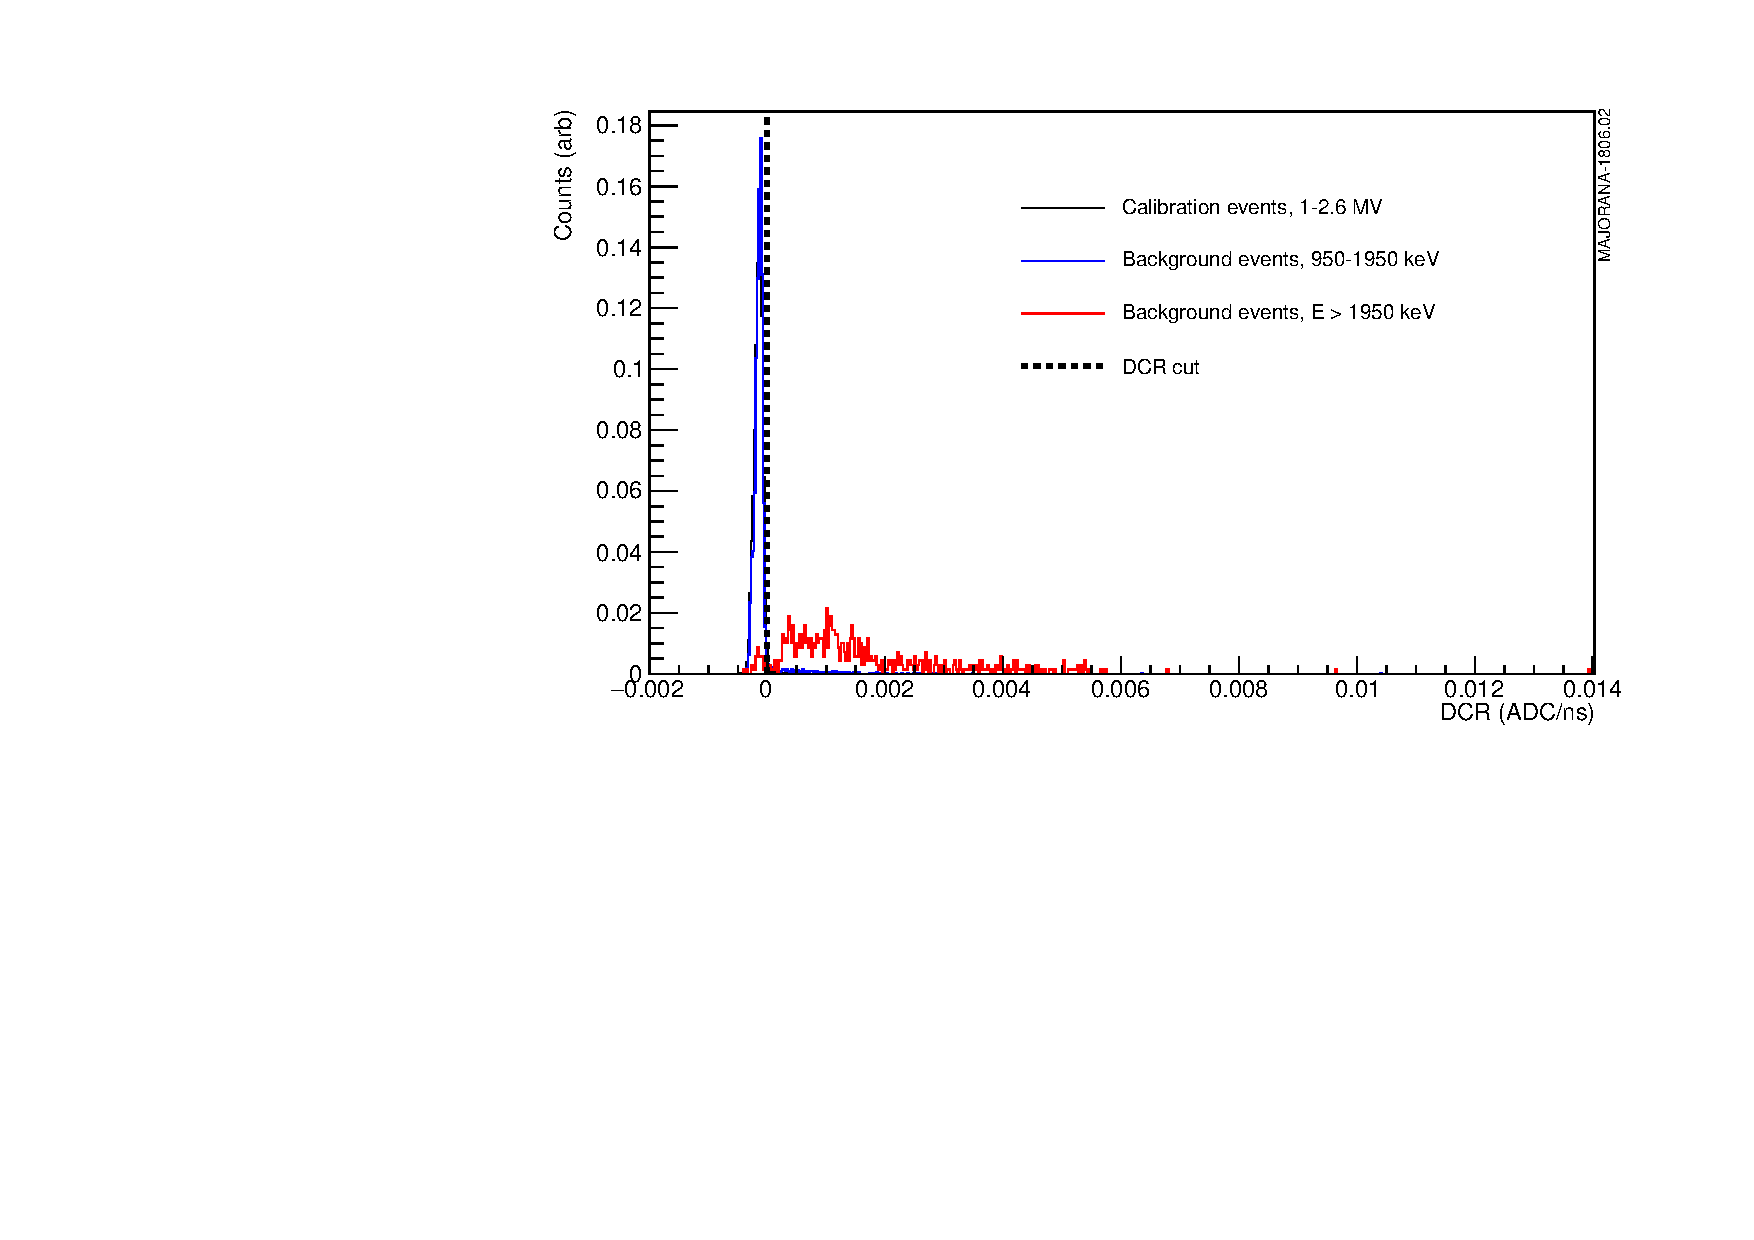
\includegraphics[width=0.54\textwidth]{DCRspectrum}}
  \caption[Surface alpha cut]{\label{fig:dcr}
    Left: A bulk event (black) compared with a DCR event (red) after pole-zero correction. The slope of the DCR event is used to tag it as a surface event.\\
    Right: The distribution of the DCR parameter, which measures the slope of the falling tail of waveforms. The high energy background events (red) are mostly $\alpha$s incident on the passivated surface. The calibration (black) and lower energy events (blue) are mostly $\gamma$s in the bulk of the detector. Surface events can be cut based on their larger DCR values.
  }
\end{figure}

Additional backgrounds in the \MJD can potentially come from $\beta$- and $\alpha$ particles incident on the surface of the HPGe detectors.
Because these are charged particles, they will be absorbed within $\sim1$~mm ($\beta$s) or $\sim.1~\mu$m ($\alpha$s) of the detector surface.
The $p^+$ and $n^+$ detector surfaces have a $\sim1.1$~mm thick lithiated layer that is dead (i.e.~virtually no charge is collected from events in this layer), meaning that these surfaces are insensitive to incident charged particles.
A passivation layer between these contacts, however, has a thickness of $\sim0.1 \mu$m, and holes created near this surface are strongly trapped.
These holes are rereleased on a time scale much longer than the trapezoidal filter time, with the result that a highly degraded energy is measured
As a result, $\alpha$ particles with energies of 3-9~MeV can be read with energies at or near the 2.039~MeV Q-value of $\beta\beta$-decay.
Some of these rereleased holes, however, are collectected within the $20-40~\mu$s window recorded by the GRETINA cards, a phenomenon referred to as Delayed Charge Recovery (DCR).
DCR can be measured by checking for a reduction in the slope of the falling tail of a waveform (or, equivalently, we would see a slow rise in the pole-zero corrected waveform instead of a flat top).
Figure~\ref{fig:dcr} shows a comparison between a DCR waveform and a bulk waveform, and the values of the DCR parameter for surface $\alpha$ events and bulk $\gamma$ events.
This cut rejects most $\alpha$ particles while keeping $\sim99\%$ of \znbb events.

\section{\MJD\ Software} \label{sec:mjsw}
The \textsc{Majorana} uses a suite of software, developed either independantly or in conjunction with other physics collaborations.
This section will give a brief overview of the software packages in use, their purpose, and their hierarchy.
The primary language for this software is \cpp, unless noted otherwise.
Aspects of this software depend on the ROOT object oriented data storage and analysis framework\cite{rootcern}, fftw3, a fast fourier transform package \cite{fftw3}, the CLHEP high energy physics library\cite{clhep}, and \geant, a simulation\cite{geant2003}.
Figure~\ref{fig:swhierarchy} shows the dependancies and hierarchy of the \MJD\ software.
\begin{figure}
  \centering
  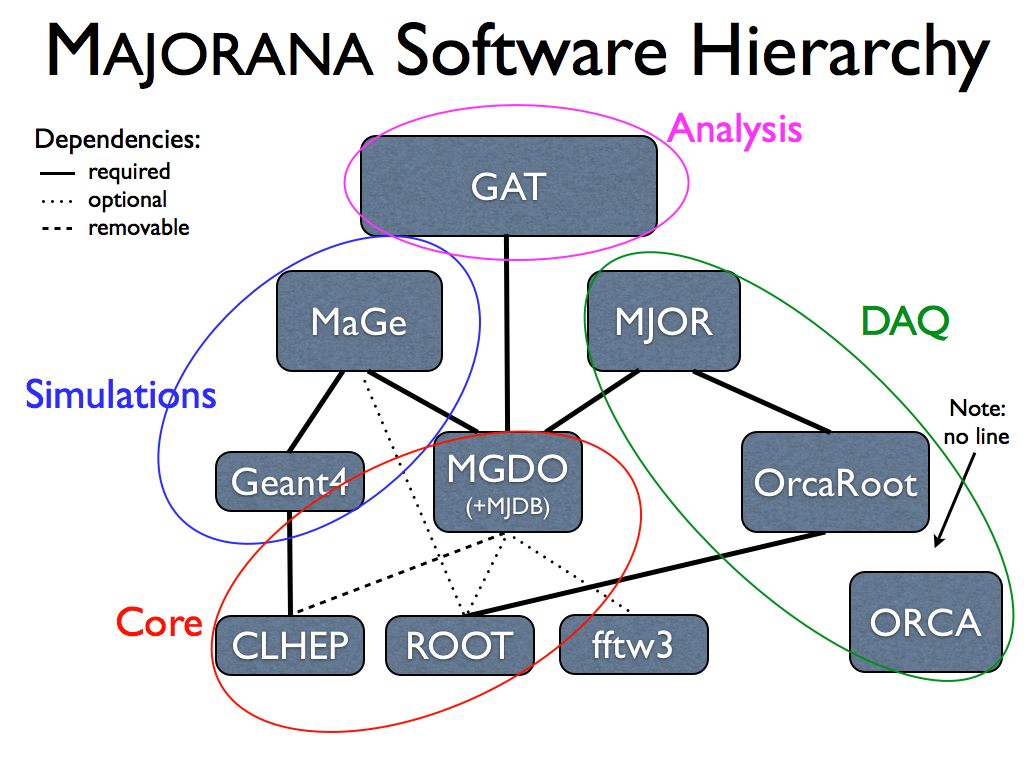
\includegraphics[width=\textwidth]{SoftwareHierarchy}
  \caption[\MJD\ software hierarchy]{\label{fig:swhierarchy}
    A diagram of the dependancies between the software libraries used for the \MJD.
  }
\end{figure}

\subsection{DAQ}
The DAQ hardware is managed and read out by the Object-oriented Real-time Control and Acquisition (ORCA) software, an object oriented DAQ framework written in Objective-C\cite{orca}.
ORCA supports a wide variety of digitizers, including the GRETINA cards and Caen QDC and scaler cards used by the \MJD.
A single computer runs an instance of ORCA that collects data from all of these cards (with the exception of Summer 2016, when two computers ran separate instances of ORCA, one for each module).
ORCA writes data packets written by the various cards to binary files, which uploaded to various \MJD\ computing systems.
Data is divided into runs, which typically last an hour in length for background runs and $\sim5$~minutes for calibration runs.
The various cards are read asynchronously by ORCA.
Between data runs, cards are not reinitialized and continue to record data; as a result, 100\% livetime is achieved during normal operations.
ORCA also supports readout of a variety of other devices that are used for environmental monitoring of the Davis Campus, and is capable of pushing these readings to an online database for access outside of the laboratory.

\subsection{MGDO}
The Majorana-Gerda Data Objects (MGDO) is a software library that is maintained by both the \MJ\ and \Gerda\ collaborations\cite{mgdo}.
MGDO contains objects for storing waveforms, data from various digitizer cards, and run information that are compatible with ROOT's \texttt{TTree}, a data storage structure.
MGDO also contains objects to perform various waveform transformations that are used in digitital signal processing.

\subsection{The Event Builder}\label{sec:eventbuilder}
The MJOR library contains the \MJ\ Event Builder, which converts the binary ORCA files into MGDO data storage objects and writes those objects to a ROOT \texttt{TTree}.
Because the ORCA readout is asynchronous, the event builder is also responsible for sorting events in time order and combining simultaneous waveforms into events.
Waveforms within a $4~\mu$s window are combined; this is a rolling window, meaning that if a waveform is within $4~\mu$s of any other waveform in the event, it will be added.
Events containing multiple detectors can be rejected for the \znbb\ analysis since \znbb\ is an inherently single-site event.
The event builder also performs some basic data quality checks, known colloquially as ``Garbage checks,'' and removes any unphysical events or events with some unreadable or incorrect data.
The event builder records events from both the HPGe detectors, read by the GRETINA cards, and from the muon veto system, read by the Caen QDC and Scaler cards.
The ROOT files produced by the event builder are known as build files.
Appendix~\ref{app:eventbuilder} contains an in depth description of the event builder.

\subsection{GAT}
The Germanium Analysis Toolkit (GAT) is a software framework for performing various analyses on the \MJD.
GAT performs the various digital waveform transformations necessary to compute the signal processing parameters described in Section~\ref{sec:mjprocessing}.
GAT records these parameters in a separate file, called a Gatified file, which is used for data analysis.
In addition, GAT produces skim files, which contain only events that pass additional data quality checks and only a single channel (between high and low gain) from each detector for each event.
One example of events that are removed by data quality checks are events that occur during liquid nitrogen dewar fills, which last $\sim15$~minutes and cause periods of high electronic noise.
Another example is events that are cut by the muon veto system, as described in Section~\ref{sec:muonveto}.
Finally, skim files are produced to include only runs and detectors that are determined to be high quality.
GAT also contains software suites to perform other analyses for the \MJD, including the \znbb\ analysis, the excited state decay analysis described in this document, and energy calibrations.

\subsection{\Mage}
The Majorana Gerda (\Mage) simulation package is used to perform simulations of the \MJD\cite{mage2011}.
It is described in detail in Chapter~\ref{ch:sims}.

\section{Recent Results}
Based on the analysis described in this chapter, the \MJD\ has produced a limit on the half-life of \znbb\ in \Ge{76}.
So far, two results have been published: one with $\sim$10~kg-y of data\cite{mjd2018}, and one with $\sim$26~kg-y of data\cite{mjd2019}, which will be discussed in this section.
Further data releases will be performed once per year until the decommissioning of the \MJD, expected in 2020.

\subsection{Data Taking and Blinding}
Module~1 began recording data on June 26, 2015 and has been in continuous operation since December 31, 2015.
Module~2 began recording data on August 25, 2016.
The data is divided into 6~numbered datasets (abbreviated DS\#) based on the configuration of the detectors and the DAQ system.
DS5 is further subdivided into DS5a, DS5b and DS5c.
The main differences between the datasets are as follows:
\begin{itemize}
\item DS0: Data taken with module~1 only, prior to the installation of the inner copper shield. This dataset has elevated backgrounds.
\item DS1: Data taken with module~1 after installation of the inner copper shield, and repairs to electronic components that resulted in a greater number of active detectors.
\item DS2: Data taken with module~1 using the digitizer multi-sampling described in Section~\ref{sec:signalelectronics}.
\item DS3: Data taken with module~1 after installation of module~2. Multi-sampling was disabled for DS3.
\item DS4: Data taken with module~2, simultaneously to DS3. Separate instances of ORCA were run for DS3 and DS4.
\item DS5a: Data taken with modules~1 and~2 using a single instance of ORCA. Data taken during this period had elevated noise due to poor detector grounding. As a result, the energy resolution and cut performance is worse for this DS than others.
\item DS5b: Data taken with both modules after improving detector grounding. This dataset ended when the \MJD\ had finished taking $\sim10$~kg-y of unblinded data for the initial data release.
\item DS5c: Continuation of DS5b, after the 10~kg-y cutoff.
\item DS6a: Data taken with both modules, with multi-sampling enabled. This dataset ended with the second data release of $\sim26$~kg-y of data.
\end{itemize}
The \MJD\ has continued recording data since the end of DS6a.

The \MJD\ follows a statistical blinding scheme, in which 75\% of data is administratively blinded and inaccessible to analysts in the \MJ\ collaboration.
The remaining 25\% of data is accessible and is used to test the analysis tools and parameters.
Implementation of this scheme is accomplished by alternating between 31~hours of background runs that are unblinded and 93~hours that are blinded.
Unblinding is performed in several stages.
First, only events with energies excluding the 1950-2350~keV region around the Q-value, low energy events and multi-detector events, all of which are used for various \MJD\ analyses.
This data is used to perform run and detector selection, and to verify the data cleaning cuts.
After verification, further data is unblinded individually for various analyses after a collaboration-wide review of the techniques.

\subsection{Analysis}
\begin{table}[h]
  \centering
  \caption[Summary of datasets]{\label{tab:dsresults}
    Summary of key parameters for each dataset.
  }
  \footnotesize
  \begin{tabular}{|cc|rr|rrrr|r|}
  \hline
  \makecell{Data\\Set} & \makecell{Start\\Date} & \makecell{Active Enr\\Mass (kg)} & \makecell{Exposure\\(kg-y)} & $\epsilon_{AE}~(\%)$ & $\epsilon_{DCR}~(\%)$ & $\epsilon_{cont}~(\%)$ & $\epsilon_{tot}~(\%)$ & \makecell{$N T \epsilon_{tot}\epsilon_{res}$\\$10^{24}$ atom-y} \\
  \hline
  DS0 & 6/26/15 & 10.69(16) & 1.26(02) & 90.1$_{-3.5}^{+3.2}$ & 98.9$_{-0.2}^{+0.9}$ & 90.8(11) & 80.8$_{-3.3}^{+3.1}$ & $6.34_{-0.27}^{+0.25}$ \\
  DS1 & 12/31/15 & 11.90(17) & 2.32(04) & 90.1$_{-4.0}^{+3.6}$ & 99.1$_{-0.5}^{+1.0}$& 90.9(11) & 81.1$_{-3.8}^{+3.5}$ & $11.82_{-0.58}^{+0.53}$ \\
  DS2 & 5/24/16 & 11.31(16) & 1.22(02) & 90.3$_{-3.7}^{+3.5}$ & 98.6$_{-0.5}^{+1.1}$& 90.9(11) & 80.9$_{-3.5}^{+3.4}$ & $6.24_{-0.29}^{+0.28}$ \\
  DS3 & 8/25/16 & 12.63(19) & 1.01(01) & 90.0$_{-3.1}^{+3.0}$ & 99.0$_{-0.3}^{+1.0}$ & 90.9(11) & 80.9$_{-3.0}^{+3.0}$ & $5.18_{-0.20}^{+0.20}$ \\
  DS4 & 8/25/16 & 5.47(08) & 0.28(00) & 90.0$_{-3.4}^{+3.1}$ & 99.2$_{-0.2}^{+1.1}$ & 90.8(10) & 80.9$_{-3.2}^{+3.0}$ & $1.47_{-0.06}^{+0.06}$ \\
  DS5a & 10/13/16 & 17.48(25) & 3.45(05) & 90.0$_{-3.6}^{+3.4}$ & 96.9$_{-1.3}^{+1.3}$ & 90.9(13) & 79.2$_{-3.5}^{+3.4}$ & $17.17_{-0.79}^{+0.76}$ \\
  DS5b & 1/27/17 & 18.44(26) & 1.85(03) & 90.0$_{-3.3}^{+3.1}$ & 98.5$_{-0.5}^{+1.4}$& 90.9(13) & 80.5$_{-3.2}^{+3.2}$ & $9.46_{-0.39}^{+0.39}$ \\
  DS5c & 3/17/17 &  18.44(26) & 1.97(03) & 90.0$_{-3.3}^{+3.1}$ & 98.5$_{-0.3}^{+1.2}$ & 90.8(11) & 80.6$_{-3.1}^{+3.1}$ &  10.31$_{-0.47}^{+0.47}$ \\
  DS6a & 5/11/17 &  18.44(26) & 12.67(19) & 90.1$_{-3.2}^{+3.2}$ & $99.0_{-0.2}^{+0.8}$ & 90.8(11) & 81.1$_{-3.0}^{+3.0}$ & 65.10$_{-2.92}^{+2.92}$ \\
  \hline
  \multicolumn{2}{|l|}{Total (DS0-6)} & & 26.02(53) & & & & & 133.1$\pm$6.3 \\
  \multicolumn{2}{|l|}{Total (DS1-4,5b-6)} & & 21.31(41) & & & & & 110.0$\pm$5.1 \\
  \hline
\end{tabular}

\end{table}
An independant analysis is performed of each dataset.
Table~\ref{tab:dsresults} contains a summary of the configuration, exposure, and detection efficiencies for each dataset.
For each detector, the active isotopic mass is computed, which is the mass of \Ge{76} that is in the bulk region of a detector, excluding dead layers (see Section~\ref{sec:dcr}.
The dead layer volume is computed based on simulations, following the procedure to be outlined in Section~\ref{sec:deadlayers}.
The total exposure for each dataset is computed by totalling the product of the active mass of each detector and the total livetime of each detector.
The detector livetime excludes runs for which that detector was disabled, time periods cut by the LN fill cut or muon veto cut, and detector deadtime, which is estimated as described in Section~\ref{sec:DT}.
The detection efficiency for this analysis is defined as the fraction of \znbb\ events originating in the active region of an active detector that is contained in the region of interest selected for the peak search.
The region of interest is selected by optimizing the detection efficiency with respect to the background acceptance, following a similar procedure to that described in Section~\ref{sec:roiopt}, and results in an ROI efficiency of $\epsilon_{res}\sim0.900\pm0.007$, with slight variations between DSs.
The cut officencies of AvsE ($\epsilon_{AE}$) and DCR ($\epsilon_{DCR}$) are calculated using the techniques described in sections~\ref{sec:avse} and~\ref{sec:dcr}.
The containment efficiency ($\epsilon_{cont}$) accounts for events that occur in the transition region between the dead layer and the bulk of the detector, where there is partial energy loss that pulls the event out of the ROI.

\begin{figure}
  \centering
  \subfloat[Full background spectrum]{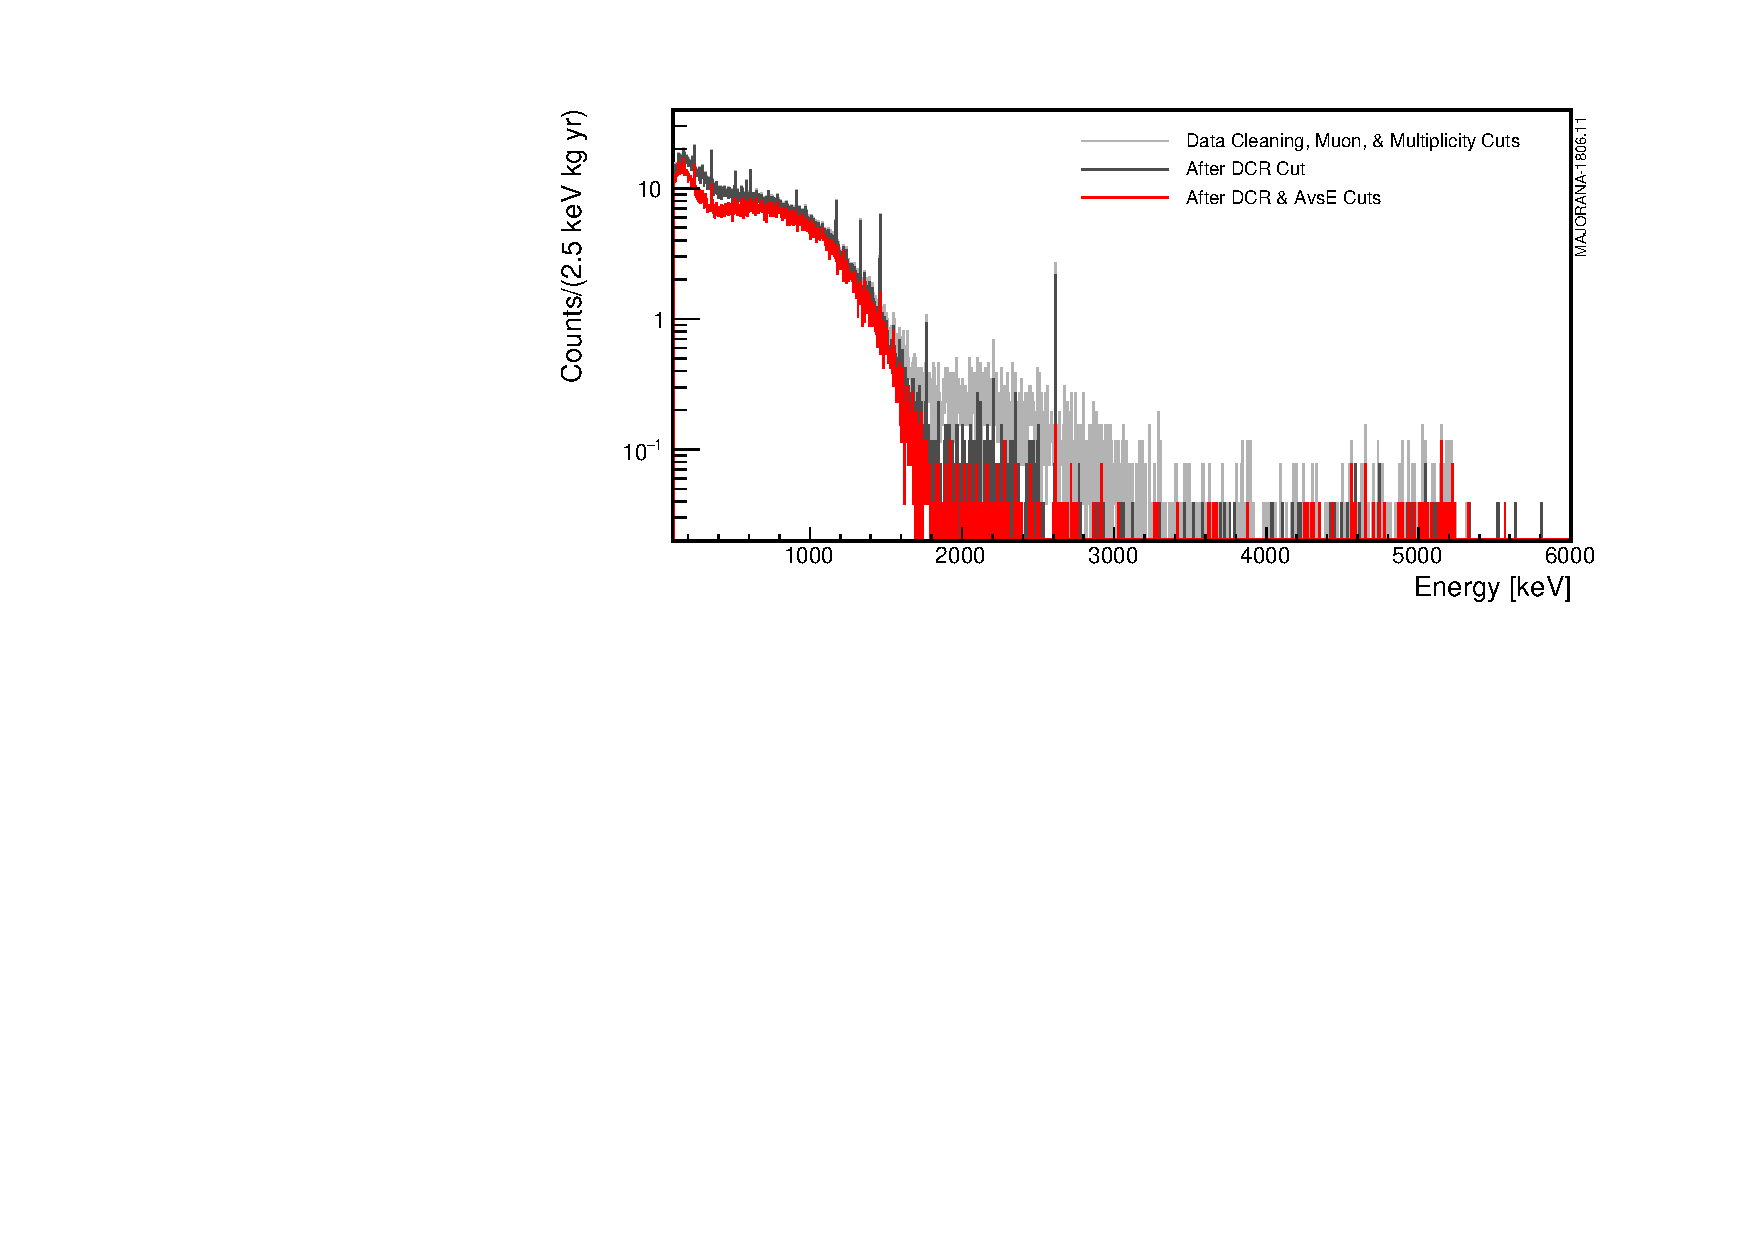
\includegraphics[height=4.5cm]{mjdbgcuts}}
  \subfloat[ROI background spectrum]{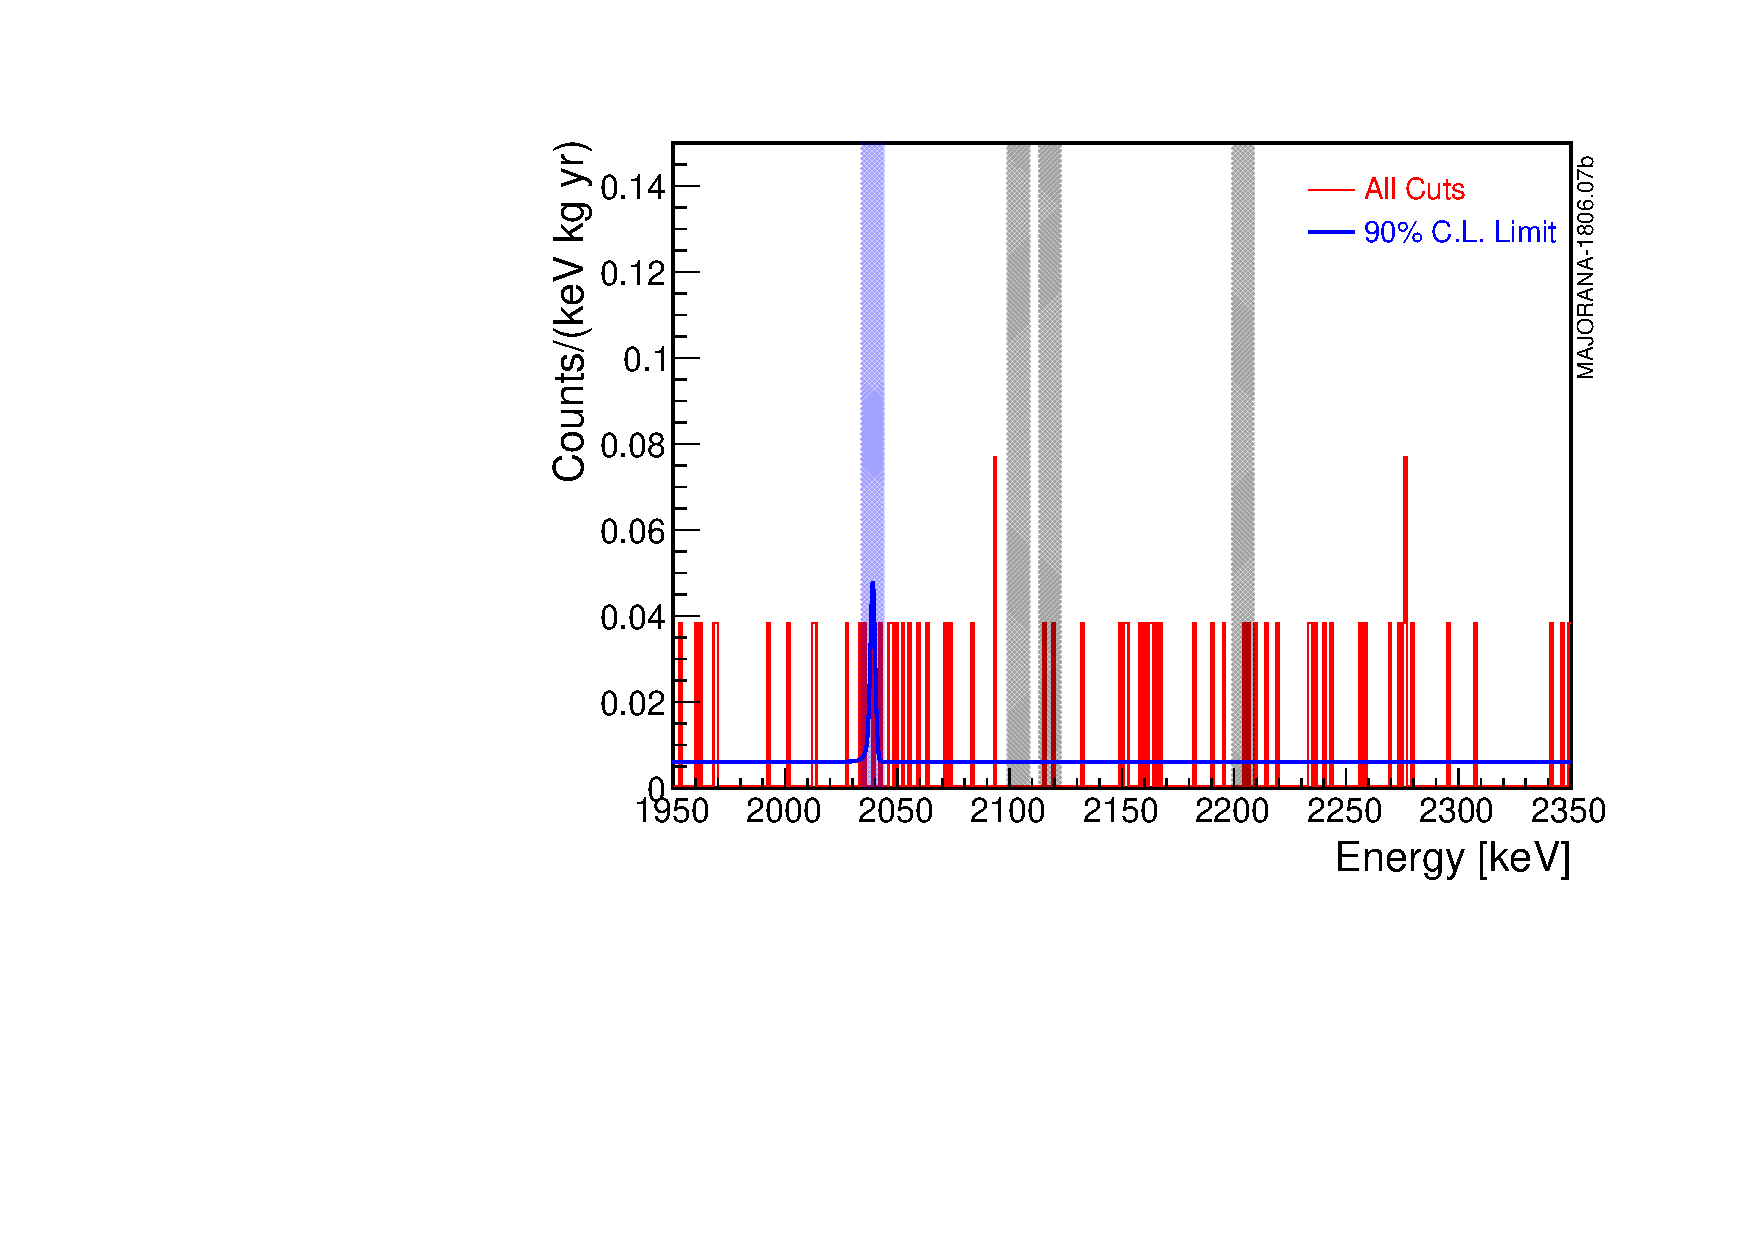
\includegraphics[height=4.5cm]{mjdbgroi}}
  \caption[\MJD\ background spectrum]{\label{mjdbgspectrum}
    The \MJD\ background spectrum for datasets 0-6a. Left: the full energy range, with cuts applied sequentially. Right: the 1950-2350~keV bacgkround region of interest spectrum after applying all cuts. The blue band is the signal ROI, and the blue curve represents the flat background with a peak with amplitude equal to the 90\% confidence limit.
  }
\end{figure}
After applying all cuts, we measure the background spectrum shown in Figure~\ref{mjdbgspectrum}.
The background index is estimated assuming a flat background in the 1950-2350~keV range, excluding regions around the known 2103~keV, 2117~keV and 2204~keV $\gamma$ peaks.
The measured background index across all datasets is $6.1\pm0.8\cdot10^{-3}$~cts/(keV-kg-y).
This corresponds to $15.4\pm2.0$ cts/(FWHM-t-y), using a 4.13~keV optimal ROI.
If we exclude high background datasets (DS0 due to the lack of inner copper shield, and DS5a due to the high noise), we measure a background index of $11.9\pm2.0$ cts/(FWHM-t-y).
Table~\ref{tab:dsbgidx} lists the background indexes broken down by dataset.
This background index falls short of the 3~ct/(FWHM-t-y) goal set for the \MJD, most likely due to \Th{232} chain contamination in excess of the predicted activity based on material assays.
\begin{table}[h]
  \centering
  \caption[Summary of datasets]{\label{tab:dsbgidx}
    Background index and optimized ROI width for each dataset.
  }
  \footnotesize
  \begin{tabular}{|r|crcc|}
  \hline
  \makecell{Dataset} & \makecell{Window\\Counts} & \makecell{BG Index\\($10^{-3}$~cts)} & \makecell{ROI\\(keV)}   & \makecell{ROI BG\\(cts)} \\
  \hline
  DS0  & 11 & $24.3_{-7.0}^{+8.4}$ & 3.93 & 0.120 \\
  DS1  &  5 &  $6.0_{-2.7}^{+3.4}$ & 4.21 & 0.058 \\
  DS2  &  2 &  $4.6_{-2.9}^{+5.1}$ & 4.34 & 0.024 \\
  DS3  &  0 &              $<$3.6 & 4.39 & 0.000 \\
  DS4  &  0 &             $<$12.7 & 4.25 & 0.000 \\
  DS5a & 10 &  $8.0_{-2.6}^{+3.1}$ & 4.49 & 0.125 \\
  DS5b &  0 &              $<$1.9 & 4.33 & 0.000 \\
  DS5c &  5 &   $7.0_{-3.2}^{+4.0}$ & 4.37 & 0.061 \\
  DS6a & 24 &   $5.3_{-1.0}^{+1.2}$ & 3.93 & 0.262 \\
  \hline
  Total & 57 & $6.1\pm0.8$  & 4.13 & 0.653 \\
  DS1-4,5b-6 & 36 & $4.7\pm0.8$ & 4.14 & 0.529 \\
  \hline
\end{tabular}

\end{table}

A poisson counting sideband analysis is performed, with 1~event in the ROI and 57 events in the $\sim350$~keV wide background ROI.
The half-life limit is determined using
\begin{equation}
  T_{1/2}^{0\nu}>\frac{\mathrm{ln}(2)NT\epsilon_{tot}\epsilon_{res}}{\hat{S}(n_{ROI}, \langle B\rangle)}
\end{equation}
where $NT\epsilon_{tot}\epsilon_{res}$ is shown in Table~\ref{tab:dsresults}, and $\hat{S}(n_{ROI}, \langle B\rangle, CL)$ is an estimator for the upper limit on the number of observed counts at confidence limit CL with $n_{ROI}$ counts and $\langle B\rangle$ expected backgrounds in the ROI.
For this result, the Feldman-Cousins estimator\cite{feldmancousins} is used with confidence level of 90\%, yielding a half-life lower limit for \Ge{76} \znbb\ of $2.5\cdot10^{25}$~y.
Other estimators have also been used and are quoted in reference~\cite{mjd2019}.
Monto Carlo simulations were performed to measure the median sensitivity at 90\% CL at $>4.8\cdot10^{25}$~y.
This half-life limit corresponds to a range of upper limits on $\langle m_{\beta\beta}\rangle$ of $(200--433)$~meV.

\section{Future Searches for \Ge{76} \znbb} \label{sec:legend}
The \MJD\ and \Gerda\ experiments are the two most sensitive searches for \znbb\ in \Ge{76} to date.
\Gerda\ has achieved a leading half-life limit of $9\cdot10^{25}$~y (90\% CL) from 82.4~kg-y of exposure\cite{gerda}.
The \MJD\ and \Gerda\ have achieved the two lowest background indexes of any \znbb\ searches, at 11.9~cts/(FWHM-t-y) for the \MJD\ and 2.1~cts/(FWHM-t-y) for \Gerda.
These low backgrounds have been achieved using differing, but complementary techniques.
\Gerda\ has achieved its low background rate largely by submerging an array of enriched HPGe detectors in liquid Argon (lAr) (see Figure~\ref{fig:legend200}.
This lAr veto acts as both passive and active shielding, since it is instrumented with photo-multiplier tubes and can detect scintillation light when a background event interacts inside the lAr.
The \MJD\ has achieved low backgrounds thanks to its ultra-clean materials, particularly the electroformed copper, superior energy resolution and improved PSA techniques.
The energy resolution and PSA improvements are enabled by the low noise LMFE electronics, which are mounted directly next to the detectors.

\begin{figure}
  \centering
  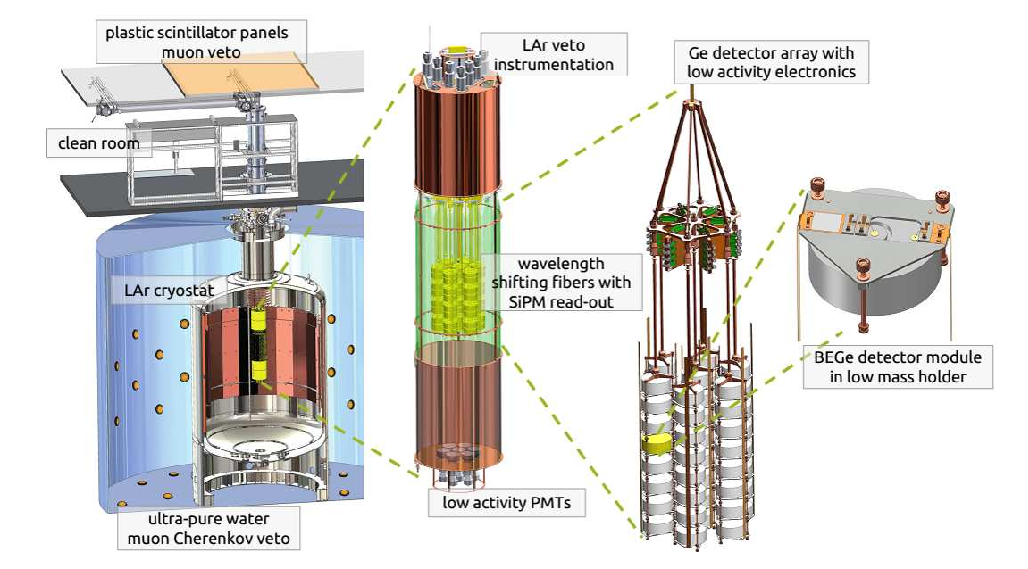
\includegraphics[width=0.8\textwidth]{legend200}
  \caption[\Gerda\ experimental design]{\label{fig:legend200}
    The components of the \Gerda\ experiment. These components will be reused for LEGEND-200, with additional HPGe detectors. Image from Gusev talk at LEGEND collaboration meeting in May 2017.
  }
\end{figure}
The \MJ\ and \Gerda\ collaborations have combined to form the LEGEND collaboration, with the plan of building a tonne-scale array of enriched PPC HPGe detectors\cite{legend}.
LEGEND will combine the background techniques demonstrated by the \MJD\ and \Gerda\ experiments and is currently undergoing active R\&D efforts to further reduce backgrounds.
Currently, two stages are planned for LEGEND.
LEGEND-200 is a 200~kg array of detectors that will utilize the existing \Gerda\ infrastructure at Gran Sasso National Laboratory (LNGS) in Italy, shown in Figure~\ref{fig:legend200}, with construction expected to begin in 2020.
In addition to the existing enriched HPGe detectors in use for both expirements, new detectors using an inverted-coaxial geometry which will have similar performance to the \MJD\ Ortec detectors, but even higher mass.
Low mass electronics based on the LMFE design will be implemented, offering improved noise performance.
The background goal for LEGEND-200 is $<0.6$~cts/(ROI-t-y), which is expected to be feasible based on simulations of the array with the previously mentioned improvements in the \Gerda\ lAr shield.
After collecting $\sim1$~t-y of exposure, LEGEND-200 is expected to have a sensitivity to \Ge{76} \znbb\ of $>10^{27}$~y at 90\% CL.

\begin{figure}
  \centering
  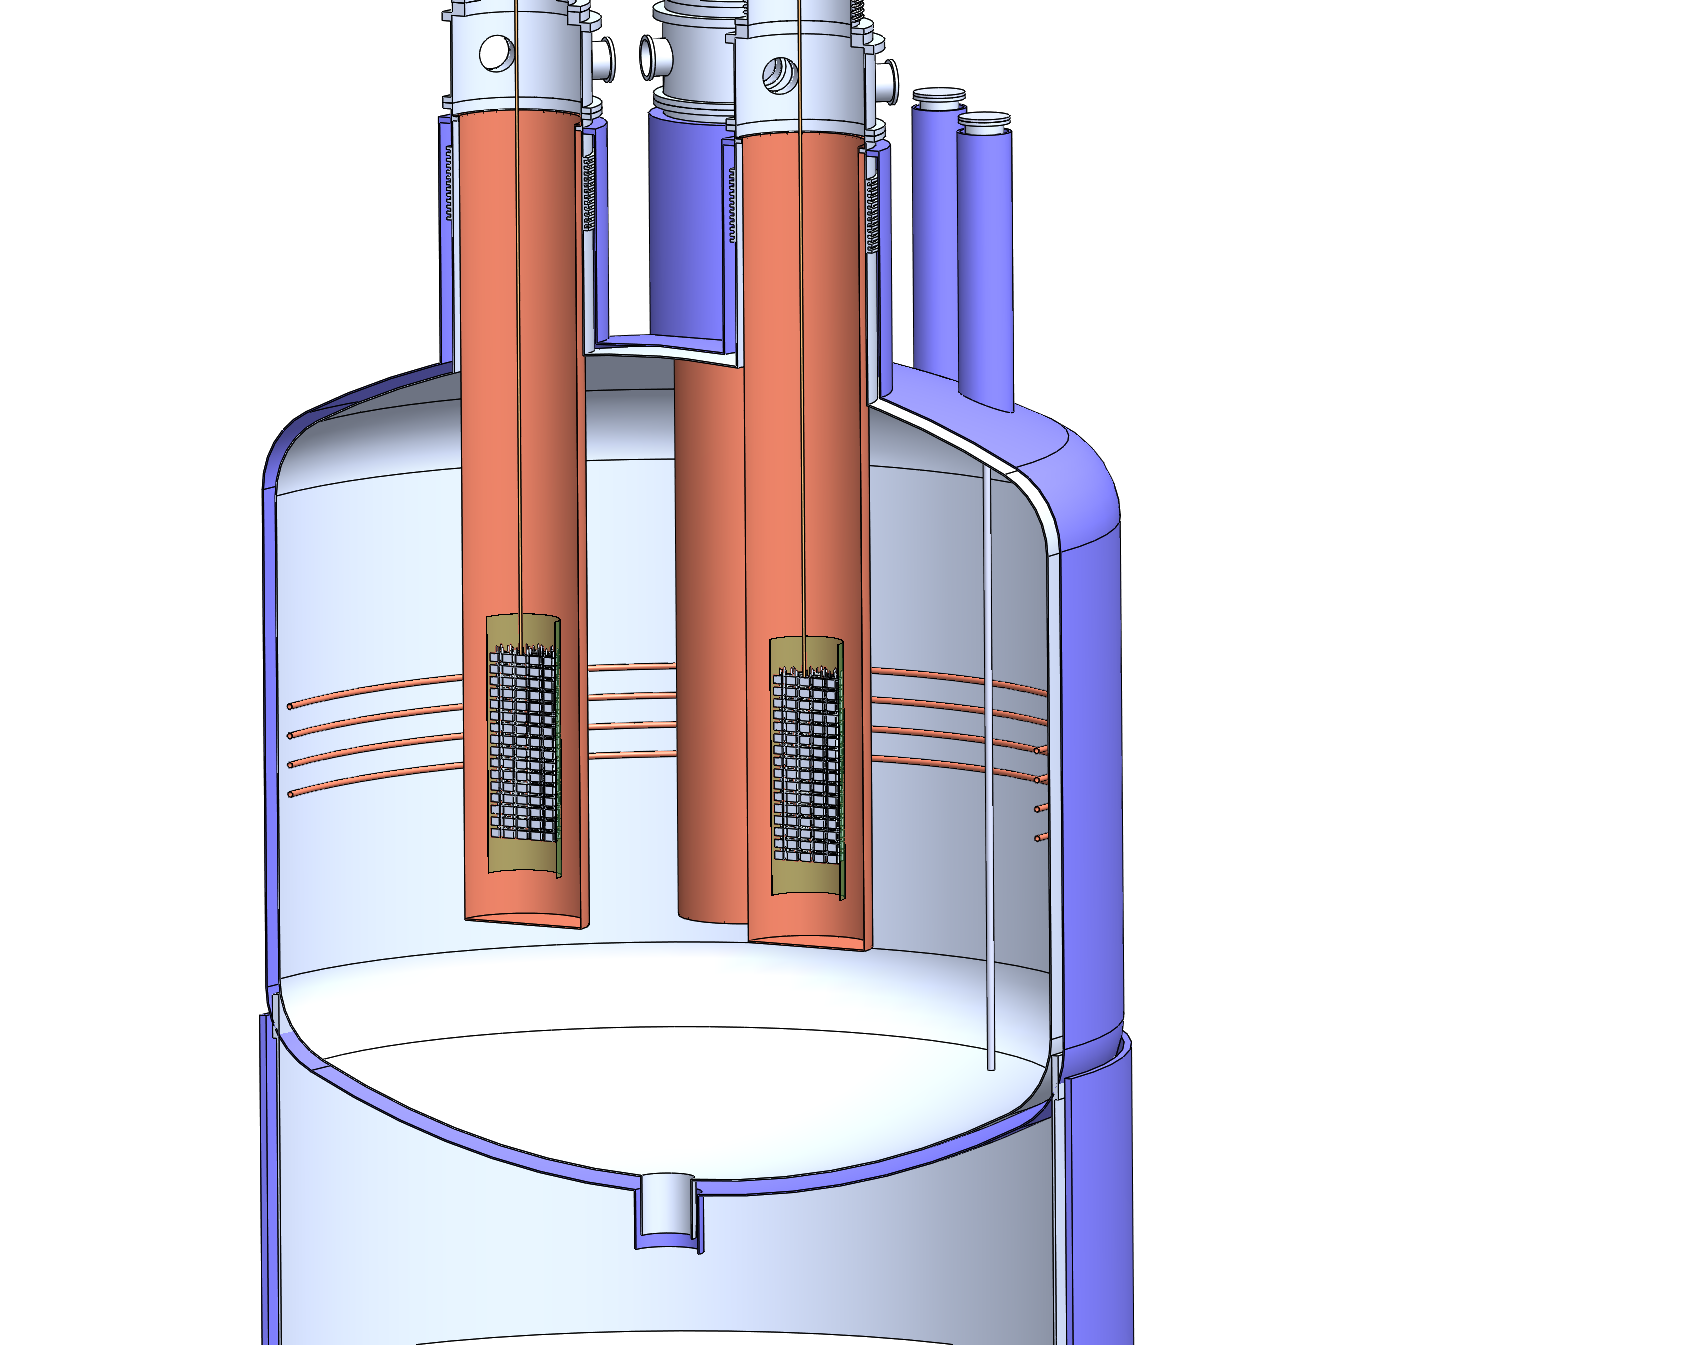
\includegraphics[width=0.5\textwidth]{legend1000}
  \caption[Legend-1000 experimental design]{\label{legend1000}
    A baseline design plan for the LEGEND-1000 experiment.
  }
\end{figure}
LEGEND-1000 is a planned 1~tonne experiment that is currently undergoing active R\&D.
A baseline design for LEGEND-1000, based on the \Gerda\ and LEGEND-200 designs, is shown in Figure~\ref{legend1000}.
In addition to the improvements implemented for LEGEND-200, LEGEND-1000 will use underground electroformed copper, and clean materials that are under development.
LEGEND-1000 will likely be housed in a laboratory with greater overburden than LNGS, reducing muon induced backgrounds.
Low background lAr from underground sources will also be used, reducing backgrounds from cosmogenically activated isotopes such as the \iso{42}{Ar}--\iso{42}{K}--\iso{42}{Ca} chain.
Based on these improvements, a background index of $<0.1$~cts/(FWHM-t-y) is expected, enabling a sensitivity to \Ge{76} \znbb\ of $>10^{27}$~y at 90\% CL with 10~t-y of exposure.

\onlyinsubfile{
  \bibliographystyle{unsrt}
  \bibliography{../main}
}
\end{document}
